\documentclass[journal,article,submit,pdftex,moreauthors]{Definitions/mdpi} 

\Title{Development of R\&R Shoes E-commerce Platform with Machine Learning-Based Recommendation System}

\TitleCitation{Development of R&R Shoes E-commerce Platform with Machine
Learning-Based Recommendation System}

\newcommand{\orcidauthorA}{0000-0000-0000-000X}

\Author{Mahendra Kirana M.B $^{1}$, Henokh Abhinaya Tjahjadi $^{1}$, Ammar Tyo Pasaribu $^{1}$, Muhammad Aditya Permana $^{1}$, Muh.Yusuf Fikry $^{1}$, Andi Alisha Faiqihah $^{1}$}

\AuthorNames{Mahendra Kirana M.B , Henokh Abhinaya Tjahjadi , Ammar Tyo Pasaribu , Muhammad Aditya Permana , Muh.Yusuf Fikry , Andi Alisha Faiqihah}

\AuthorCitation{B, M.; Tjahjadi, H.; Pasaribu, A.; Permana, M.; Fikry, M.; Faiqihah, A.}

\address{%
$^{1}$ \quad Universitas Hasanuddin; mbmk22h@student.unhas.ac.id, Tjahjadiha22h@student.unhas.ac.id, 
pasaribuat22h@student.unhas.ac.id, 
Permanama22h@student.unhas.ac.id, 
Fikrymy22h@student.unhas.ac.id, 
Faiqihahaa22h@student.unhas.ac.id}

\corres{Correspondence: pasaribuat22h@student.unhas.ac.id; Tel.: +62-895-6201-63633 (F.L.)}

\abstrak{
Website e-commerce sepatu R\&R dikembangkan dengan mengintegrasikan sistem rekomendasi berbasis machine learning untuk meningkatkan pengalaman berbelanja pengguna. Penelitian ini menjelaskan pengembangan platform e-commerce yang menggunakan algoritma Non-negative Matrix Factorization (NMF) untuk menganalisis pola interaksi pengguna dan memberikan rekomendasi produk yang dipersonalisasi. Data dikumpulkan dari interaksi pengguna seperti view, wishlist, cart, dan pembelian, serta informasi produk dari berbagai kategori sepatu. Platform ini dibangun menggunakan React.js untuk frontend dan Flask untuk backend, dengan sistem rekomendasi yang dilatih untuk mengenali pola preferensi pengguna. Hasil evaluasi menunjukkan tingkat presisi dan recall yang baik dalam memberikan rekomendasi produk yang relevan. Dengan demikian, platform ini tidak hanya memudahkan pengguna dalam menemukan produk yang sesuai dengan preferensi mereka, tetapi juga membantu meningkatkan potensi konversi penjualan melalui rekomendasi yang dipersonalisasi.}

\katakunci{Machine Learning; e-commerce; Sepatu}

\abstract{
The R\&R shoes e-commerce website was developed by integrating a machine learning-based recommendation system to enhance the user shopping experience. This research describes the development of an e-commerce platform that utilizes the Non-negative Matrix Factorization (NMF) algorithm to analyze user interaction patterns and provide personalized product recommendations. Data is collected from user interactions such as views, wishlists, carts, and purchases, as well as product information from various shoe categories. The platform is built using React.js for frontend and Flask for backend, with a recommendation system trained to recognize user preference patterns. Evaluation results show good precision and recall rates in providing relevant product recommendations. Thus, this platform not only makes it easier for users to find products that match their preferences but also helps increase sales conversion potential through personalized recommendations.}

\keyword{Machine Learning; e-commerce; Shoes}

\begin{document}

% ... existing code ...


\section{Project Charter}

\subsubsection{Project Description}
Website e-commerce sepatu R\&R merupakan platform penjualan sepatu online yang mengintegrasikan sistem rekomendasi berbasis machine learning. Proyek ini dirancang untuk meningkatkan pengalaman berbelanja pengguna dengan memberikan rekomendasi produk yang dipersonalisasi menggunakan algoritma Non-negative Matrix Factorization (NMF). Platform ini mengotomatisasi proses rekomendasi produk berdasarkan pola interaksi pengguna seperti view, wishlist, cart, dan pembelian. Dengan menerapkan teknologi modern seperti React.js untuk frontend dan Flask untuk backend, sistem ini tidak hanya menyediakan antarmuka yang responsif tetapi juga memproses data secara efisien untuk menghasilkan rekomendasi yang akurat.
\subsubsection{Pembagian Role Tim}
\begin{table}[ht]
\centering
\begin{tabular}{|c|c|}
\hline
\textbf{Nama} & \textbf{Role} \\
\hline
Mahendra Kirana M.B & Project Manager \\
Henokh Abhinaya Tjahjadi & Backend Developer \\
Ammar Tyo Pasaribu & Backend Developer \\
Muh.Yusuf Fikry & Frontend Developer \\
Andi Alisha Faiqihah & Frontend Developer \\
Muhammad Aditya Permana & UI/UX Designer  \\
\hline
\end{tabular}
\captionsetup{justification=centering}
\caption{Pembagian \textit{Role} Tim}
\end{table}


\subsubsection{SMART Question}
Website e-commerce sepatu R\&R dirancang untuk meningkatkan pengalaman berbelanja pengguna dengan mengintegrasikan sistem rekomendasi berbasis machine learning. Platform ini menggunakan teknologi Non-negative Matrix Factorization (NMF) untuk menganalisis pola interaksi pengguna dan memberikan rekomendasi produk yang dipersonalisasi. Dengan menggunakan data interaksi pengguna seperti view, wishlist, cart, dan pembelian, sistem dapat memahami preferensi pengguna dan memberikan rekomendasi yang relevan.

Inisiatif ini mendukung upaya peningkatan konversi penjualan melalui personalisasi pengalaman berbelanja, dengan memastikan bahwa setiap pengguna mendapatkan rekomendasi yang sesuai dengan preferensi mereka. Dengan menggunakan teknologi modern seperti React.js untuk frontend dan Flask untuk backend, platform ini diharapkan dapat memberikan layanan yang responsif dan efisien. Pada akhirnya, website ini ditargetkan untuk dapat dirilis dalam versi beta yang fungsional dalam waktu 16 minggu, menyediakan solusi e-commerce yang inovatif dengan fitur rekomendasi yang cerdas.

\subsubsection{Alat / Tools}
\begin{enumerate}[left=2em]
    \item React.js
    \item Flask
    \item SQLite
    \item Python (Scikit-learn)
    \item Git
    \item Figma
\end{enumerate}

\subsubsection{Target User}
\begin{enumerate}[left=2em]
    \item Pembeli sepatu online
    \item Pengguna yang mencari rekomendasi sepatu
    \item Pengguna yang sering berbelanja sepatu online
\end{enumerate}

\subsection{Situasi dan Kondisi Sekarang}
Saat ini, banyak platform e-commerce sepatu yang beroperasi secara konvensional tanpa sistem rekomendasi yang efektif. Beberapa tantangan yang dihadapi:

\begin{itemize}[left=2em]
    \item \textbf{Pengalaman berbelanja yang tidak personal:} Pengguna kesulitan menemukan produk yang sesuai dengan preferensi mereka
    \item \textbf{Keterbatasan dalam personalisasi:} Sistem rekomendasi yang ada masih belum optimal dalam memahami preferensi pengguna
    \item \textbf{Konversi penjualan yang belum maksimal:} Kurangnya rekomendasi yang tepat menyebabkan potensi penjualan tidak tercapai
\end{itemize}

\subsection{Proyek Sebelumnya yang Mirip}
Platform e-commerce dengan sistem rekomendasi telah banyak berkembang di Indonesia, dengan beberapa pemain besar seperti Tokopedia, Shopee, dan Bukalapak yang telah menerapkan sistem rekomendasi canggih dalam platform mereka. Di tingkat global, Amazon telah menjadi pionir dalam pengembangan sistem rekomendasi e-commerce dengan algoritma item-to-item collaborative filtering mereka yang terkenal.

Sistem rekomendasi yang diterapkan oleh platform-platform tersebut umumnya menggunakan kombinasi dari collaborative filtering dan content-based filtering untuk menganalisis pola belanja dan preferensi pengguna. Namun, sebagian besar platform ini menerapkan sistem rekomendasi untuk berbagai kategori produk secara umum, tidak terfokus pada kategori spesifik seperti sepatu.

R\&R mengambil pendekatan yang berbeda dengan berfokus khusus pada kategori sepatu dan mengimplementasikan algoritma Non-negative Matrix Factorization (NMF) yang lebih sederhana namun efektif. Pendekatan ini memungkinkan personalisasi yang lebih spesifik untuk kategori produk tertentu, dengan mempertimbangkan karakteristik unik dari perilaku pembelian sepatu. Dengan fokus yang lebih spesifik ini, R\&R dapat memberikan rekomendasi yang lebih relevan dan akurat untuk pengguna yang mencari produk sepatu.



\section{Methods}
\subsection{Data Collection}

Pengumpulan data dilakukan melalui penyusunan manual dan pencatatan interaksi pengguna untuk membangun dataset produk sepatu serta dataset interaksi pengguna. Langkah-langkah yang dilakukan adalah sebagai berikut:


    \item \textbf{Identifikasi Sumber Data}:
    \begin{itemize}
        \item Dataset sepatu disusun dengan memasukkan produk dari lima kategori utama: formal, sport, heels, boots, dan casual.
        \item Setiap kategori terdiri dari 10 jenis sepatu berbeda, sehingga total terdapat 50 produk sepatu dalam dataset.
    \end{itemize}
    
    \item \textbf{Pembuatan Dataset Produk}:
    \begin{itemize}
        \item Dataset produk sepatu dibuat secara manual dengan menentukan nama sepatu, kategori, dan informasi dasar lainnya.
        \item Masing-masing sepatu diberi \textit{id\_sepatu} sebagai identitas unik untuk digunakan dalam pemetaan data interaksi.
    \end{itemize}
    
    \item \textbf{Pengumpulan Data Interaksi Pengguna}:
    \begin{itemize}
        \item Dataset interaksi pengguna (\textit{user\_interaction}) berisi data yang menunjukkan aktivitas pengguna pada setiap produk sepatu di situs.
        \item Data interaksi ini meliputi \textit{id\_user}, \textit{id\_sepatu}, dan jenis \textit{interaction}, seperti \textit{view}, \textit{cart}, \textit{buy}, dan \textit{wishlist}, yang dicatat berdasarkan aktivitas pengguna.
    \end{itemize}
    
    \item \textbf{Penyimpanan Data}:
    \begin{itemize}
        \item Setiap data interaksi pengguna disimpan dalam format yang terstruktur di dalam dataset \textit{user\_interaction}.
        \item Data ini diatur agar mudah diakses oleh model rekomendasi untuk melatih sistem berdasarkan aktivitas pengguna yang relevan.
    \end{itemize}


% ... existing code ...

\subsection{Data Explanation}
Pada proyek ini, terdapat dua dataset utama yang digunakan untuk melatih model rekomendasi sepatu, yaitu Dataset Produk dan Dataset Interaksi Pengguna. Berikut adalah penjelasan lebih lanjut tentang kedua dataset ini:

\subsubsection{Dataset Produk}
Dataset produk mencakup informasi dasar mengenai sepatu yang tersedia di platform e-commerce. Setiap entri dalam dataset ini mewakili satu produk sepatu dan berisi atribut sebagai berikut:

\begin{itemize}
    \item \textbf{id\_sepatu}: ID unik untuk setiap sepatu. ID ini berfungsi sebagai pengidentifikasi yang akan dipetakan dalam dataset interaksi pengguna.
    \item \textbf{kategori}: Jenis atau kategori sepatu, seperti "formal", "sport", "heels", "boots", atau "casual". Kategori ini membantu mengelompokkan sepatu berdasarkan gaya dan fungsi.
    \item \textbf{nama\_sepatu}: Nama atau model sepatu, yang dapat memberikan konteks bagi pengguna terkait produk yang ditawarkan.
\end{itemize}

Contoh entri dataset:

\begin{table}[h]
\centering
\begin{tabular}{|c|c|c|}
\hline
\textbf{id\_sepatu} & \textbf{kategori} & \textbf{nama\_sepatu} \\ \hline
1 & formal & Wirken Oxford \\ \hline
2 & sport & Ardiles Nfinity Burst \\ \hline
3 & heels & Celline Heels \\ \hline
4 & boots & Parabellum COBRA \\ \hline
5 & casual & Asics Gel Sonoma SE \\ \hline
\end{tabular}
\end{table}

Dataset produk ini penting untuk memberikan konteks bagi sistem rekomendasi mengenai karakteristik dasar dari setiap produk.

\subsubsection{Dataset Interaksi Pengguna (user\_interaction)}
Dataset ini berisi data interaksi antara pengguna dan produk di platform, yang mencakup berbagai aktivitas pengguna yang relevan. Atribut-atribut dalam dataset interaksi pengguna meliputi:

\begin{itemize}
    \item \textbf{id\_user}: ID unik pengguna yang melakukan interaksi. Atribut ini membantu dalam pelacakan aktivitas individual pengguna.
    \item \textbf{id\_sepatu}: ID sepatu yang diinteraksikan oleh pengguna, menghubungkan dataset ini dengan dataset produk.
    \item \textbf{interaction\_type}: Jenis interaksi yang dilakukan pengguna pada produk. Nilai ini dapat berupa:
    \begin{itemize}
        \item view (melihat produk)
        \item cart (memasukkan ke keranjang)
        \item buy (membeli produk)
        \item wishlist (menambahkan ke daftar keinginan)
    \end{itemize}
    Jenis interaksi ini digunakan untuk melatih model dalam memahami tingkat ketertarikan pengguna terhadap suatu produk.
\end{itemize}

Contoh entri dataset:

\begin{table}[h]
\centering
\begin{tabular}{|c|c|c|}
\hline
\textbf{id\_user} & \textbf{id\_sepatu} & \textbf{interaction} \\ \hline
1 & 12 & view \\ \hline
1 & 2 & buy \\ \hline
2 & 43 & wishlist \\ \hline
3 & 24 & cart \\ \hline
4 & 15 & view \\ \hline
\end{tabular}
\end{table}

Dataset interaksi pengguna ini penting karena menjadi sumber utama dalam melatih model rekomendasi. Berdasarkan data ini, model dapat belajar pola preferensi pengguna untuk memberikan rekomendasi yang sesuai.

Dengan kedua dataset ini, model rekomendasi dapat dilatih untuk mengenali pola interaksi pengguna dan menawarkan produk yang relevan, meningkatkan pengalaman pengguna serta potensi konversi di platform e-commerce.


\subsection{Theoretical Model}
Model teoretis yang digunakan dalam proyek ini adalah \textit{Non-negative Matrix Factorization} (NMF), yang merupakan teknik \textit{Collaborative Filtering}. NMF dipilih karena kemampuannya dalam mengidentifikasi pola tersembunyi dalam data interaksi pengguna-produk dan menghasilkan rekomendasi yang dipersonalisasi. Berikut adalah penjelasan detail mengenai model teoretis yang digunakan:

\begin{enumerate}
    \item \textbf{Dasar Teori NMF}:
    \begin{itemize}
        \item NMF adalah teknik dekomposisi matriks yang memfaktorkan matriks non-negatif \(V\) menjadi dua matriks non-negatif \(W\) dan \(H\), di mana \(V \approx WH\).
        \item Dalam konteks sistem rekomendasi:
        \begin{itemize}
            \item \(V\) adalah matriks interaksi pengguna-produk
            \item \(W\) adalah matriks yang merepresentasikan hubungan pengguna dengan fitur laten
            \item \(H\) adalah matriks yang merepresentasikan hubungan fitur laten dengan produk
        \end{itemize}
        \item Batasan non-negatif pada matriks memastikan interpretabilitas yang lebih baik dari fitur laten yang dihasilkan.
    \end{itemize}

    \item \textbf{Formulasi Matematis}:
    \begin{itemize}
        \item Objective Function:
        \[
        \min_{W,H} \|V - WH\|_F^2 \text{ subject to } W,H \geq 0
        \]
        \item Di mana \(\|\cdot\|_F\) adalah norma Frobenius
        \item Dimensi matriks:
        \begin{itemize}
            \item \(V \in \mathbb{R}^{m \times n}\)
            \item \(W \in \mathbb{R}^{m \times k}\)
            \item \(H \in \mathbb{R}^{k \times n}\)
            \item \(k\) adalah jumlah fitur laten yang dipilih
        \end{itemize}
    \end{itemize}

    \item \textbf{Keunggulan Model NMF}:
    \begin{itemize}
        \item \textit{Interpretabilitas}: Hasil faktorisasi dapat diinterpretasikan secara langsung karena semua nilai non-negatif.
        \item \textit{Skalabilitas}: Dapat menangani dataset besar dengan efisien karena proses faktorisasi yang relatif sederhana.
        \item \textit{Sparsitas}: Mampu menangani data yang sparse, yang umum dalam data interaksi pengguna-produk.
        \item \textit{Fleksibilitas}: Dapat diintegrasikan dengan berbagai jenis data interaksi (view, wishlist, cart, buy).
    \end{itemize}

    \item \textbf{Implementasi dalam Sistem Rekomendasi}:
    \begin{itemize}
        \item \textit{Representasi Data}:
        \begin{itemize}
            \item Matriks interaksi dibentuk dengan pengguna sebagai baris dan produk sebagai kolom
            \item Nilai dalam matriks merepresentasikan tingkat interaksi (1-4 untuk view, wishlist, cart, buy)
        \end{itemize}
        \item \textit{Proses Pembelajaran}:
        \begin{itemize}
            \item Inisialisasi random untuk matriks \(W\) dan \(H\)
            \item Iterative update rules untuk meminimalkan error rekonstruksi
            \item Konvergensi dicapai ketika perubahan error minimal
        \end{itemize}
        \item \textit{Pemberian Rekomendasi}:
        \begin{itemize}
            \item Prediksi preferensi dihitung melalui perkalian \(WH\)
            \item Top-K produk dengan nilai prediksi tertinggi direkomendasikan
        \end{itemize}
    \end{itemize}

    \item \textbf{Pertimbangan Teoretis}:
    \begin{itemize}
        \item \textit{Pemilihan Jumlah Fitur Laten}: 
        \begin{itemize}
            \item Trade-off antara kompleksitas model dan akurasi prediksi
            \item Dipilih melalui validasi silang untuk optimasi performa
        \end{itemize}
        \item \textit{Penanganan Cold Start}:
        \begin{itemize}
            \item Untuk pengguna baru: menggunakan rekomendasi berbasis popularitas
            \item Untuk produk baru: menggunakan similaritas berbasis konten
        \end{itemize}
        \item \textit{Regularisasi}:
        \begin{itemize}
            \item L2 regularization diterapkan untuk mencegah overfitting
            \item Parameter regularisasi dioptimasi melalui validasi silang
        \end{itemize}
    \end{itemize}
\end{enumerate}
\subsection{Algorithm or Model}
Pada proyek ini, sistem rekomendasi sepatu dibangun menggunakan model \textit{Non-negative Matrix Factorization} (NMF), yang merupakan teknik \textit{Collaborative Filtering}. Berikut adalah langkah-langkah dan detail dari model yang digunakan:

\begin{enumerate}
    \item \textbf{Persiapan Data}:
    \begin{itemize}
        \item \textit{Dataset Interaksi Pengguna} dan \textit{Dataset Produk} digabungkan untuk membentuk matriks pengguna-produk (\textit{user-item matrix}). Matriks ini berfungsi sebagai dasar untuk pelatihan model.
        \item Setiap jenis interaksi pengguna (seperti \textit{view}, \textit{wishlist}, \textit{cart}, dan \textit{buy}) dipetakan ke nilai numerik. Misalnya, \textit{view} diberi nilai 1, \textit{wishlist} diberi nilai 2, \textit{cart} diberi nilai 3, dan \textit{buy} diberi nilai 4. Pemetaan ini membantu dalam mengukur tingkat ketertarikan pengguna terhadap produk.
    \end{itemize}

    \item \textbf{Pembentukan Matriks}:
    \begin{itemize}
        \item Matriks pengguna-produk dibentuk dengan menggunakan nilai interaksi sebagai elemen matriks. Setiap baris mewakili pengguna, dan setiap kolom mewakili produk. Matriks ini menggambarkan hubungan antara pengguna dan produk berdasarkan interaksi yang terjadi.
        \item Nilai kosong dalam matriks diisi dengan nol untuk menunjukkan tidak adanya interaksi. Hal ini penting untuk memastikan bahwa model dapat memproses data dengan benar tanpa kesalahan.
    \end{itemize}

    \item \textbf{Pelatihan Model NMF}:
    \begin{itemize}
        \item Model NMF dilatih menggunakan matriks pengguna-produk. NMF memfaktorkan matriks ini menjadi dua matriks yang lebih kecil: matriks pengguna-fitur (\textit{W}) dan matriks fitur-produk (\textit{H}). Proses ini membantu dalam mengidentifikasi pola laten dalam data.
        \item Matriks \textit{W} merepresentasikan preferensi laten pengguna, sedangkan matriks \textit{H} merepresentasikan karakteristik laten produk. Dengan kata lain, \textit{W} menunjukkan bagaimana setiap pengguna berhubungan dengan fitur-fitur tertentu, dan \textit{H} menunjukkan bagaimana setiap produk berhubungan dengan fitur-fitur tersebut.
        \item Parameter model seperti jumlah komponen laten (\textit{n\_components}) diatur untuk mengoptimalkan hasil rekomendasi. Pemilihan parameter yang tepat sangat penting untuk meningkatkan akurasi model.
    \end{itemize}

    \item \textbf{Pemberian Rekomendasi}:
    \begin{itemize}
        \item Untuk pengguna baru, rekomendasi diberikan berdasarkan popularitas produk yang dihitung dari interaksi pengguna lain. Hal ini dilakukan karena tidak ada data interaksi sebelumnya untuk pengguna baru.
        \item Untuk pengguna yang sudah ada, skor preferensi dihitung dengan mengalikan matriks \textit{W} dan \textit{H}, dan produk dengan skor tertinggi direkomendasikan. Proses ini memungkinkan sistem untuk memberikan rekomendasi yang dipersonalisasi berdasarkan preferensi pengguna yang telah dipelajari.
    \end{itemize}

    \item \textbf{Evaluasi Model}:
    \begin{itemize}
        \item Model dievaluasi menggunakan metrik seperti \textit{Precision@k}, \textit{Recall@k}, dan \textit{Mean Average Precision (MAP)@k} untuk mengukur akurasi rekomendasi. Evaluasi ini penting untuk memastikan bahwa model memberikan rekomendasi yang relevan.
        \item Precision mengukur proporsi rekomendasi yang relevan dari semua rekomendasi yang diberikan, sedangkan recall mengukur proporsi item relevan yang berhasil direkomendasikan dari semua item relevan yang tersedia. MAP memberikan gambaran keseluruhan tentang akurasi model dalam memberikan rekomendasi yang relevan.
    \end{itemize}
\end{enumerate}

Dengan pendekatan ini, sistem rekomendasi dapat memberikan saran produk yang lebih relevan kepada pengguna, meningkatkan pengalaman pengguna dan potensi konversi di platform e-commerce.



\subsection{Testing (Procedures and Metrics)}
Pengujian sistem rekomendasi dilakukan untuk memastikan bahwa model memberikan rekomendasi yang akurat dan relevan. Berikut adalah prosedur dan metrik yang digunakan dalam pengujian:

\begin{enumerate}
    \item \textbf{Prosedur Pengujian}:
    \begin{itemize}
        \item \textit{Split Data}: Dataset dibagi menjadi data pelatihan dan data pengujian. Data pelatihan digunakan untuk melatih model, sedangkan data pengujian digunakan untuk mengevaluasi kinerja model.
        \item \textit{Pelatihan Model}: Model dilatih menggunakan data pelatihan dengan parameter yang telah ditentukan.
        \item \textit{Prediksi Rekomendasi}: Model menghasilkan rekomendasi untuk pengguna dalam data pengujian.
    \end{itemize}

    \item \textbf{Metrik Evaluasi}:
    \begin{itemize}
        \item \textit{Precision@k}: Mengukur proporsi rekomendasi yang relevan dari semua rekomendasi yang diberikan hingga posisi ke-k. Precision yang tinggi menunjukkan bahwa model memberikan rekomendasi yang relevan.
        \item \textit{Recall@k}: Mengukur proporsi item relevan yang berhasil direkomendasikan dari semua item relevan yang tersedia hingga posisi ke-k. Recall yang tinggi menunjukkan bahwa model mampu menangkap sebagian besar item relevan.
        \item \textit{Mean Average Precision (MAP)@k}: Menghitung rata-rata presisi pada berbagai level cut-off dalam daftar rekomendasi hingga posisi ke-k. MAP memberikan gambaran keseluruhan tentang akurasi model dalam memberikan rekomendasi yang relevan.
    \end{itemize}

    \item \textbf{Analisis Hasil}:
    \begin{itemize}
        \item Hasil pengujian dianalisis untuk mengidentifikasi kekuatan dan kelemahan model. Analisis ini membantu dalam mengoptimalkan model lebih lanjut.
        \item Perbandingan dilakukan antara hasil pengujian dan ekspektasi untuk memastikan bahwa model memenuhi tujuan yang diinginkan.
    \end{itemize}
\end{enumerate}

Pengujian ini memastikan bahwa sistem rekomendasi dapat memberikan saran produk yang relevan dan meningkatkan pengalaman pengguna di platform e-commerce.


% ... existing code ...
% ... existing code ...

\subsection{Evaluation Metrics}

\begin{enumerate}
    \item \textbf{Precision@K}:
    \begin{itemize}
        \item Precision pada peringkat \( K \) adalah persentase item yang direkomendasikan dalam \( K \) teratas yang relevan bagi pengguna. Precision berfokus pada relevansi dari rekomendasi dalam daftar \( K \) teratas, bukan seberapa baik rekomendasi mencakup semua item relevan. Dengan kata lain, metrik ini menjawab pertanyaan: Dari semua item yang direkomendasikan dalam \( K \) teratas, berapa banyak yang benar-benar relevan?
        \item Rumus:
        \[
        \text{Precision@K} = \frac{\text{jumlah item relevan dalam } K \text{ teratas}}{K}
        \]
        \item Contoh: Jika kita merekomendasikan 5 item dan 3 di antaranya relevan, maka Precision@5 adalah:
        \[
        \text{Precision@5} = \frac{3}{5} = 0.6
        \]
    \end{itemize}

    \item \textbf{Recall@K}:
    \begin{itemize}
        \item Recall pada peringkat \( K \) adalah proporsi item relevan yang berhasil direkomendasikan dalam \( K \) teratas. Metrik ini mengukur seberapa baik model menangkap semua item relevan dalam daftar rekomendasi, tanpa memperhitungkan jumlah item yang direkomendasikan. Recall menjawab pertanyaan: Dari semua item yang dianggap relevan oleh pengguna, berapa banyak yang muncul dalam \( K \) teratas?
        \item Rumus:
        \[
        \text{Recall@K} = \frac{\text{jumlah item relevan dalam } K \text{ teratas}}{\text{jumlah total item relevan}}
        \]
        \item Contoh: Jika seorang pengguna memiliki 10 item yang relevan tetapi hanya 3 yang muncul dalam \( K \) teratas, Recall@K adalah:
        \[
        \text{Recall@10} = \frac{3}{10} = 0.3
        \]
    \end{itemize}

    \item \textbf{Accuracy@K}:
    \begin{itemize}
        \item Dalam konteks ini, Accuracy@K mengukur persentase item yang direkomendasikan dengan benar (hit) di antara semua item relevan, khususnya dalam \( K \) teratas. Accuracy mirip dengan Recall tetapi fokus pada perbandingan jumlah item yang direkomendasikan dengan benar relatif terhadap jumlah total item relevan.
        \item Rumus:
        \[
        \text{Accuracy@K} = \frac{\text{jumlah item relevan yang direkomendasikan dalam } K \text{ teratas}}{\text{jumlah total item relevan}}
        \]
    \end{itemize}

    \item \textbf{Mean Average Precision (MAP@K)}:
    \begin{itemize}
        \item MAP@K adalah metrik yang lebih lanjut yang memperhitungkan posisi item relevan dalam daftar rekomendasi. MAP@K mengukur precision di setiap posisi dalam peringkat, lalu menghitung rata-ratanya di semua item relevan. Metrik ini berguna untuk kasus di mana urutan rekomendasi berpengaruh karena item relevan yang muncul lebih awal akan mendapatkan skor lebih tinggi.
        \item Rumus:
        \[
        \text{MAP@K} = \frac{1}{N} \sum_{i=1}^{N} \text{Average Precision@K}_{i}
        \]
        \item dengan:
        \begin{itemize}
            \item \( N \) adalah jumlah pengguna,
            \item \( \text{Average Precision@K}_{i} \) adalah rata-rata precision pada \( K \) untuk setiap pengguna.
        \end{itemize}
    \end{itemize}

    \item \textbf{Kemiripan Nilai Antara Precision dan MAP, Recall dan Accuracy}:
    \begin{itemize}
        \item Berdasarkan dataset yang terdiri dari 500 interaksi pengguna di antara 20 pengguna unik, beberapa pola dapat menjelaskan mengapa precision dan MAP cenderung serupa, dan mengapa nilai recall dan accuracy sering kali mirip.
        \item \textit{Kemiripan Precision dan MAP}: Baik Precision@K maupun MAP@K berfokus pada relevansi item dalam \( K \) teratas. Karena MAP memberi bobot lebih tinggi pada item relevan yang muncul di awal daftar rekomendasi, nilai MAP akan cenderung mirip dengan Precision jika sebagian besar item relevan selalu muncul di peringkat atas secara konsisten.
        \item \textit{Kemiripan Recall dan Accuracy}: Recall@K dan Accuracy@K keduanya mengukur seberapa baik daftar rekomendasi mencakup item relevan, meskipun dari perspektif yang sedikit berbeda. Recall adalah persentase item relevan yang muncul dalam rekomendasi, sementara akurasi, seperti yang diimplementasikan di sini, juga menghitung hit di antara item relevan.
    \end{itemize}
\end{enumerate}



\section{Problem}

Dalam pengembangan website e-commerce sepatu R\&R dengan fitur sistem rekomendasi, terdapat beberapa permasalahan utama yang perlu diselesaikan:

\subsection{Masalah Bisnis}
\begin{itemize}
    \item \textbf{Personalisasi Terbatas:} Platform e-commerce sepatu yang ada saat ini umumnya menampilkan produk yang sama untuk semua pengguna, tanpa mempertimbangkan preferensi individual.
    
    \item \textbf{Konversi Rendah:} Tanpa sistem rekomendasi yang efektif, pengguna kesulitan menemukan sepatu yang sesuai dengan preferensi mereka, yang mengakibatkan tingkat konversi penjualan yang rendah.
    
    \item \textbf{Pengalaman Pengguna:} Pengguna harus menghabiskan waktu lebih lama untuk mencari sepatu yang mereka inginkan karena tidak adanya rekomendasi yang dipersonalisasi.
\end{itemize}

\subsection{Tantangan Teknis}
\begin{itemize}
    \item \textbf{Data Interaksi Terbatas:} 
    \begin{itemize}
        \item Keterbatasan dalam mengumpulkan data interaksi pengguna yang cukup untuk melatih model rekomendasi.
        \item Dataset yang tersedia hanya mencakup 50 produk sepatu dari 5 kategori berbeda.
    \end{itemize}
    
    \item \textbf{Cold Start Problem:} 
    \begin{itemize}
        \item Kesulitan dalam memberikan rekomendasi yang akurat untuk pengguna baru yang belum memiliki riwayat interaksi.
        \item Tantangan dalam merekomendasikan produk baru yang belum memiliki data interaksi.
    \end{itemize}
    
    \item \textbf{Skalabilitas Sistem:}
    \begin{itemize}
        \item Kebutuhan untuk memproses dan menganalisis data interaksi pengguna secara real-time.
        \item Tantangan dalam memastikan performa sistem tetap optimal saat jumlah pengguna dan produk bertambah.
    \end{itemize}
\end{itemize}

\subsection{Solusi yang Diusulkan}
\begin{itemize}
    \item \textbf{Implementasi NMF:} Menggunakan algoritma Non-negative Matrix Factorization untuk sistem rekomendasi yang dapat memberikan saran produk yang dipersonalisasi berdasarkan pola interaksi pengguna.
    
    \item \textbf{Pendekatan Hybrid:} Menggabungkan rekomendasi berbasis popularitas untuk pengguna baru dengan rekomendasi personal untuk pengguna yang sudah memiliki riwayat interaksi.
    
    \item \textbf{Optimasi Frontend:} Menggunakan React.js untuk membangun antarmuka yang responsif dan mudah digunakan, memastikan pengalaman pengguna yang optimal.
\end{itemize}

\section{Intelligence System}
% ... existing code ...

\subsection{System Architecture}
Arsitektur sistem e-commerce sepatu ini dirancang untuk mendukung fitur rekomendasi yang efisien dan responsif. Sistem ini terdiri dari beberapa komponen utama yang bekerja secara sinergis untuk memberikan pengalaman pengguna yang optimal.

\begin{enumerate}
    \item \textbf{Frontend}:
    \begin{itemize}
        \item \textit{React.js} digunakan untuk membangun antarmuka pengguna yang dinamis dan interaktif. React.js dipilih karena kemampuannya dalam mengelola komponen UI yang kompleks dan memperbarui tampilan secara efisien.
        \item Komponen frontend bertanggung jawab untuk menampilkan produk, menangani interaksi pengguna seperti pencarian dan filter, serta menampilkan rekomendasi produk secara real-time.
        \item Antarmuka pengguna dirancang agar responsif dan mudah digunakan, memastikan bahwa pengguna dapat dengan mudah menemukan dan membeli produk yang mereka inginkan.
    \end{itemize}

    \item \textbf{Backend}:
    \begin{itemize}
        \item \textit{Flask} digunakan sebagai framework web untuk mengembangkan API yang menghubungkan frontend dengan database dan model rekomendasi. Flask dipilih karena kesederhanaan dan fleksibilitasnya dalam menangani permintaan HTTP.
        \item Backend bertanggung jawab untuk memproses permintaan dari frontend, seperti permintaan data produk dan interaksi pengguna, serta mengelola logika bisnis untuk rekomendasi.
        \item \textit{SQLite} digunakan sebagai database untuk menyimpan data produk dan interaksi pengguna. SQLite dipilih karena kemudahan penggunaan, integrasi yang mulus dengan Flask, dan kemampuan untuk menangani data dalam skala kecil hingga menengah.
        \item Database dirancang untuk menyimpan informasi produk, kategori, dan riwayat interaksi pengguna, yang semuanya penting untuk menghasilkan rekomendasi yang akurat.
    \end{itemize}

    \item \textbf{Model Rekomendasi}:
    \begin{itemize}
        \item Model rekomendasi dibangun menggunakan \textit{Non-negative Matrix Factorization} (NMF), yang merupakan teknik collaborative filtering. NMF digunakan untuk mengidentifikasi pola laten dalam data interaksi pengguna.
        \item Model ini diintegrasikan ke dalam backend untuk memproses data secara efisien dan memberikan rekomendasi yang dipersonalisasi kepada pengguna.
        \item Proses rekomendasi melibatkan analisis data interaksi pengguna untuk mengidentifikasi preferensi dan memberikan saran produk yang relevan, meningkatkan pengalaman belanja pengguna.
    \end{itemize}
\end{enumerate}

Arsitektur ini dirancang untuk memastikan bahwa sistem dapat menangani permintaan pengguna dengan cepat dan memberikan pengalaman belanja yang dipersonalisasi dan memuaskan. Dengan memanfaatkan teknologi modern seperti React.js dan Flask, sistem ini mampu memberikan layanan yang responsif dan efisien.

% ... existing code ...
\subsection{System Workflow}
Alur kerja sistem e-commerce sepatu R\&R dengan fitur rekomendasi terdiri dari beberapa tahapan utama yang saling terhubung:

\subsubsection{Alur Interaksi Pengguna}
\begin{enumerate}
    \item \textbf{Registrasi dan Login}:
    \begin{itemize}
        \item Pengguna baru melakukan registrasi dengan memasukkan data diri
        \item Pengguna yang sudah terdaftar dapat langsung login ke sistem
        \item Sistem memverifikasi kredensial pengguna
    \end{itemize}

    \item \textbf{Browsing Produk}:
    \begin{itemize}
        \item Pengguna dapat melihat katalog produk sepatu
        \item Sistem mencatat setiap interaksi view produk
        \item Pengguna dapat melakukan filter berdasarkan kategori
    \end{itemize}

    \item \textbf{Interaksi dengan Produk}:
    \begin{itemize}
        \item Menambahkan produk ke wishlist
        \item Memasukkan produk ke keranjang belanja
        \item Melakukan pembelian produk
        \item Setiap interaksi dicatat dalam database
    \end{itemize}
\end{enumerate}

\subsubsection{Alur Sistem Rekomendasi}
\begin{enumerate}
    \item \textbf{Pengumpulan Data}:
    \begin{itemize}
        \item Sistem mengumpulkan data interaksi pengguna secara real-time
        \item Data interaksi meliputi view, wishlist, cart, dan purchase
        \item Data disimpan dalam format terstruktur di database
    \end{itemize}

    \item \textbf{Pemrosesan Data}:
    \begin{itemize}
        \item Data interaksi dikonversi menjadi matriks user-item
        \item Sistem menerapkan pembobotan berdasarkan jenis interaksi
        \item Model NMF memproses matriks untuk menghasilkan rekomendasi
    \end{itemize}

    \item \textbf{Generasi Rekomendasi}:
    \begin{itemize}
        \item Untuk pengguna baru: rekomendasi berbasis popularitas
        \item Untuk pengguna existing: rekomendasi personal berbasis NMF
        \item Hasil rekomendasi ditampilkan di antarmuka pengguna
    \end{itemize}
\end{enumerate}

\subsubsection{Alur Backend Processing}
\begin{enumerate}
    \item \textbf{Manajemen Data}:
    \begin{itemize}
        \item Penyimpanan data produk dan interaksi di SQLite
        \item Pembaruan data secara real-time
        \item Backup dan maintenance database
    \end{itemize}

    \item \textbf{API Endpoints}:
    \begin{itemize}
        \item Endpoint untuk manajemen pengguna
        \item Endpoint untuk operasi CRUD produk
        \item Endpoint untuk sistem rekomendasi
    \end{itemize}

    \item \textbf{Response Handling}:
    \begin{itemize}
        \item Pemrosesan permintaan dari frontend
        \item Pengiriman response dalam format JSON
        \item Penanganan error dan exception
    \end{itemize}
\end{enumerate}


\subsubsection{Class Diagram}
% Penjelasan class diagram berdasarkan rincian yang diberikan
\begin{figure}[H]
    \centering
    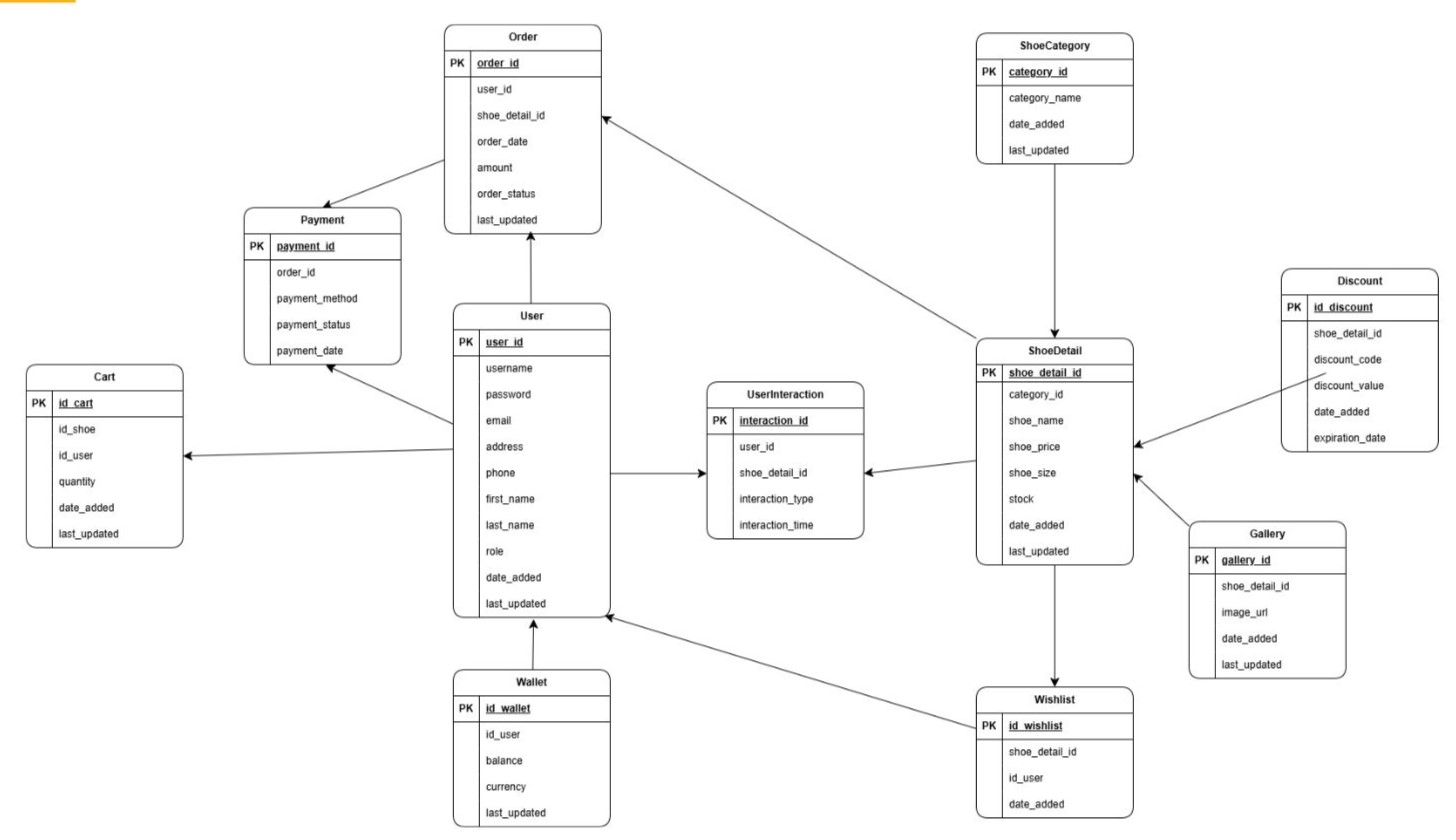
\includegraphics[width=1.0\textwidth]{images/classdiagram.jpg}
     \captionsetup{justification=centering}
    \caption{\textit{Class Diagram}}
    \label{fig:enter-label}
\end{figure}
\begin{itemize}
    \item \textbf{User Management}:
    \begin{itemize}
        \item Tabel User sebagai pusat data pengguna dengan atribut lengkap seperti username, password, email, dll.
        \item Terhubung dengan Wallet untuk manajemen saldo pengguna
        \item Memiliki relasi dengan Cart, Order, dan Wishlist untuk aktivitas pembelian
    \end{itemize}
    
    \item \textbf{Product Management}:
    \begin{itemize}
        \item Tabel ShoeDetail sebagai pusat informasi produk
        \item Terhubung dengan ShoeCategory untuk klasifikasi produk
        \item Memiliki Gallery untuk manajemen gambar produk
        \item Terintegrasi dengan Discount untuk pengelolaan promosi
    \end{itemize}
    
    \item \textbf{Transaction Management}:
    \begin{itemize}
        \item Tabel Order untuk pencatatan pembelian
        \item Terhubung dengan Payment untuk proses pembayaran
        \item Terintegrasi dengan Cart untuk proses checkout
    \end{itemize}
    
    \item \textbf{Recommendation System}:
    \begin{itemize}
        \item Tabel UserInteraction untuk mencatat aktivitas pengguna
        \item Menjadi dasar untuk sistem rekomendasi berbasis NMF
    \end{itemize}
\end{itemize}



\subsubsection{Use Case Diagram}
% Penjelasan use case diagram berdasarkan rincian yang diberikan

\begin{figure}[H]
    \centering
    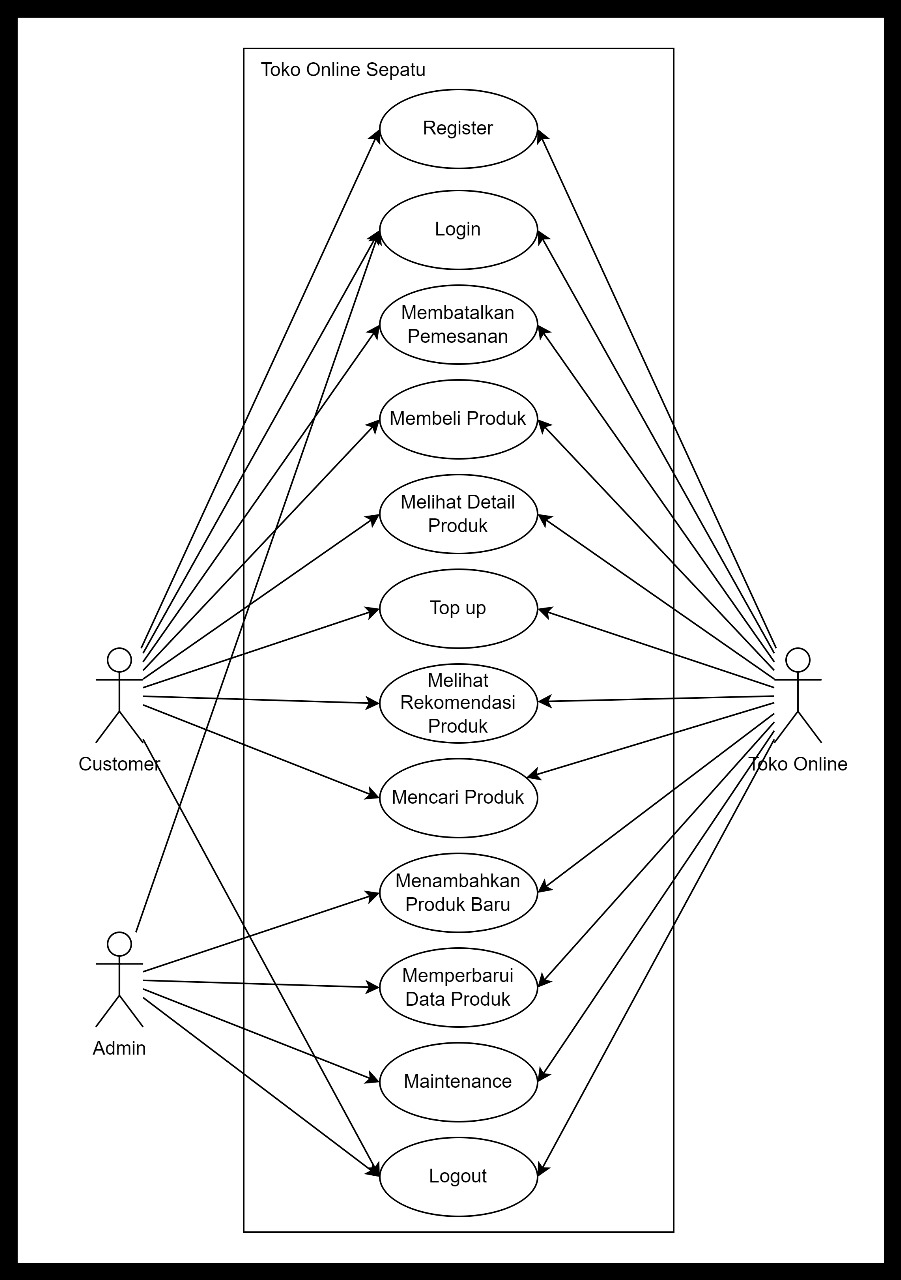
\includegraphics[width=0.8\textwidth]{images/UMLdiagram.jpeg}
     \captionsetup{justification=centering}
    \caption{\textit{UML Diagram}}
    \label{fig:enter-label}
\end{figure}
\begin{itemize}
    \item \textbf{Customer Activities}:
    \begin{itemize}
        \item Manajemen akun (register, login, logout)
        \item Aktivitas belanja (melihat produk, membeli, membatalkan pesanan)
        \item Fitur wallet (top up)
        \item Akses rekomendasi dan pencarian produk
    \end{itemize}
    
    \item \textbf{Admin Activities}:
    \begin{itemize}
        \item Manajemen produk (menambah, memperbarui)
        \item Maintenance sistem
        \item Login dan logout admin
    \end{itemize}
\end{itemize}

\subsubsection{Activity Diagrams}

\begin{figure}[H]
    \centering
    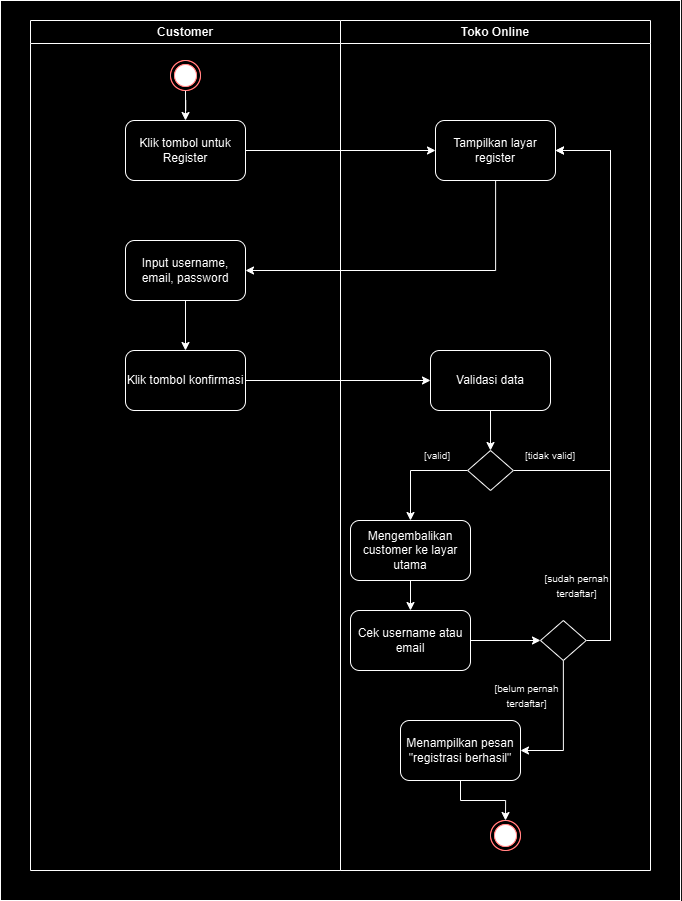
\includegraphics[width=0.7\textwidth]{images/activityregistersdiagram.png}
    \captionsetup{justification=centering}
    \caption{\textit{Activity Diagram Register}}
    \label{fig:activity-register}
\end{figure}

\begin{figure}[H]
    \centering
    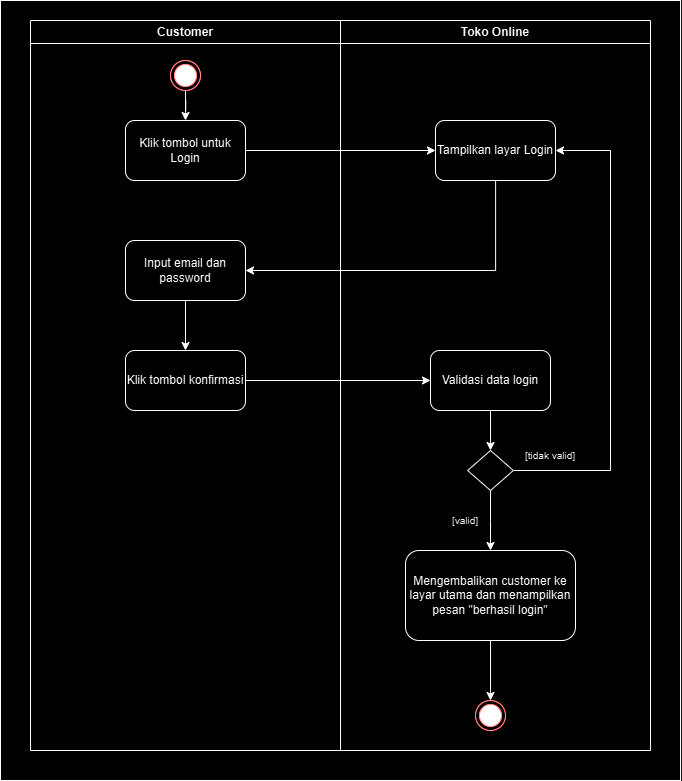
\includegraphics[width=0.7\textwidth]{images/acitivtylogindiagram.png}
    \captionsetup{justification=centering}
    \caption{\textit{Activity Diagram Login}}
    \label{fig:activity-login}
\end{figure}

\begin{figure}[H]
    \centering
    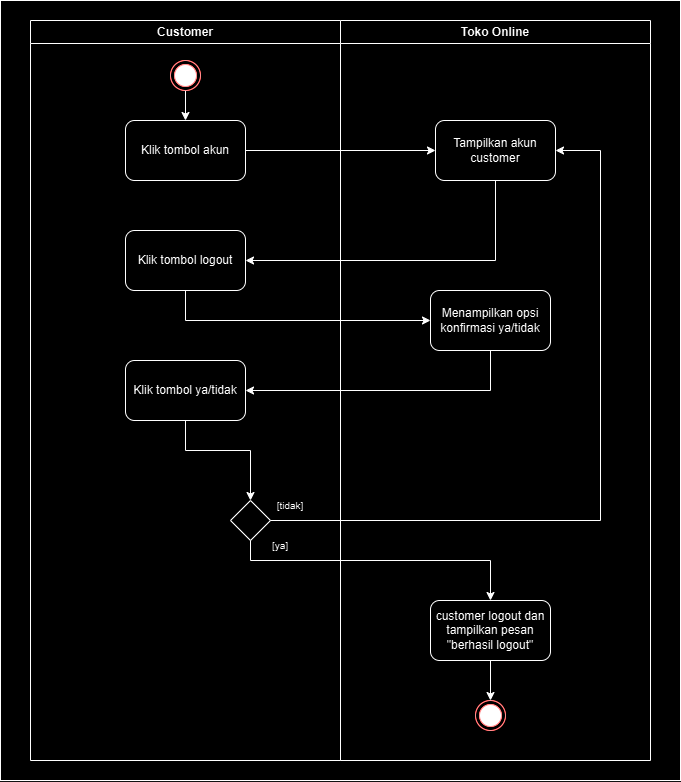
\includegraphics[width=0.7\textwidth]{images/activitylogoutdiagram.png}
    \captionsetup{justification=centering}
    \caption{\textit{Activity Diagram Logout}}
    \label{fig:activity-search}
\end{figure}

\begin{figure}[H]
    \centering
    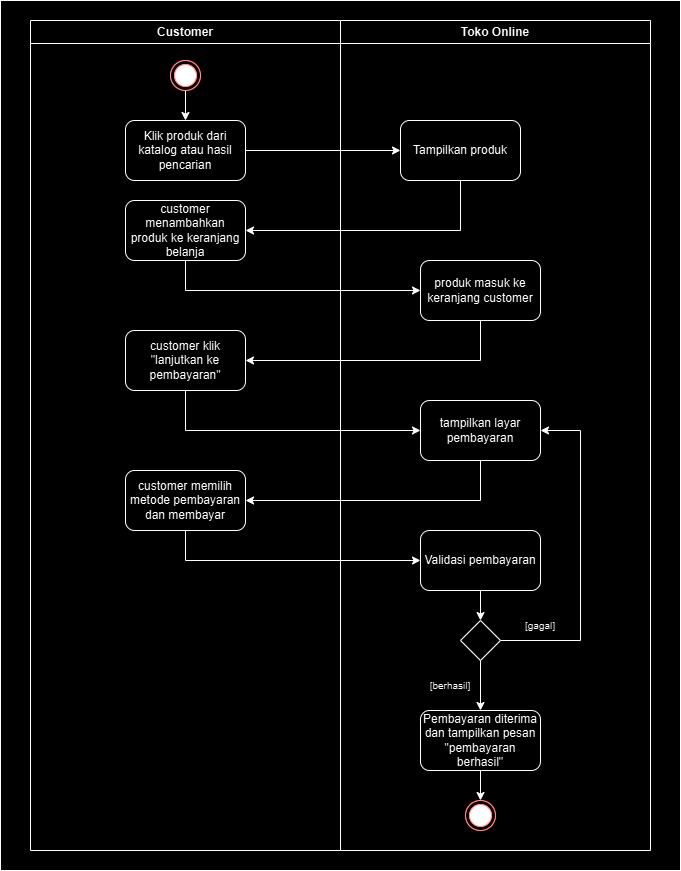
\includegraphics[width=0.7\textwidth]{images/activitymembelisepatudiagram.png}
    \captionsetup{justification=centering}
    \caption{\textit{Activity Diagram Membeli Sepatu}}
    \label{fig:activity-cart}
\end{figure}

\begin{figure}[H]
    \centering
    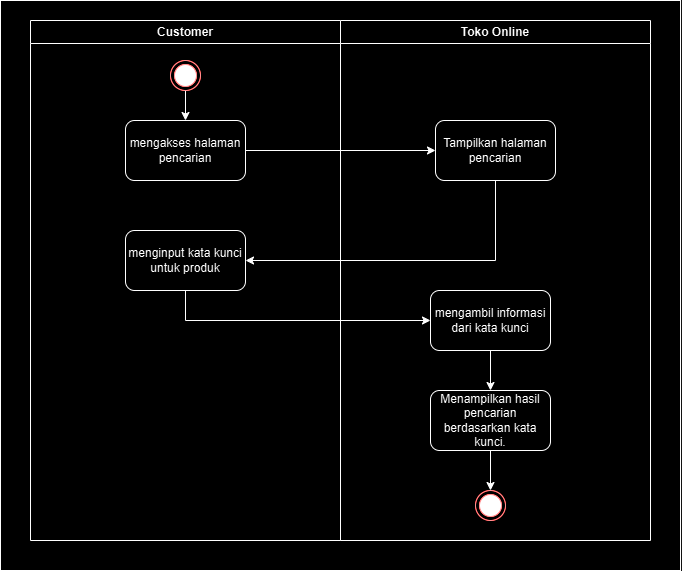
\includegraphics[width=0.7\textwidth]{images/activitysearchprodukdiagram.png}
    \captionsetup{justification=centering}
    \caption{\textit{Activity Diagram Search Sepatu}}
    \label{fig:activity-checkout}
\end{figure}

\begin{figure}[H]
    \centering
    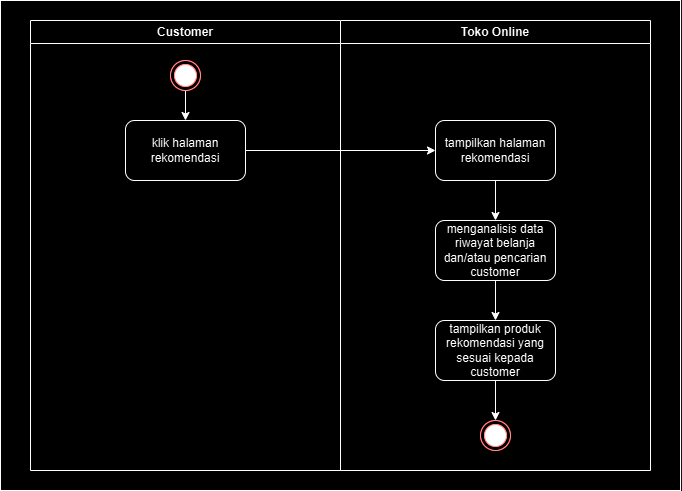
\includegraphics[width=0.7\textwidth]{images/activitylihatrekomendasidiagram.png}
    \captionsetup{justification=centering}
    \caption{\textit{Activity Diagram Rekomendasi Sepatu}}
    \label{fig:activity-payment}
\end{figure}

\begin{figure}[H]
    \centering
    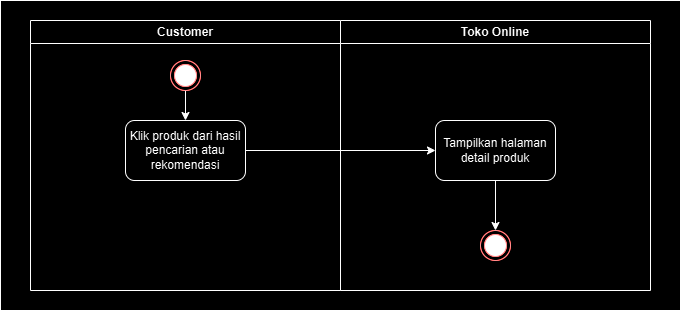
\includegraphics[width=0.7\textwidth]{images/activitylihatdetailsepatudiagram.png}
    \captionsetup{justification=centering}
    \caption{\textit{Activity Diagram Melihat Detail Sepatu}}
    \label{fig:activity-order}
\end{figure}

\begin{figure}[H]
    \centering
    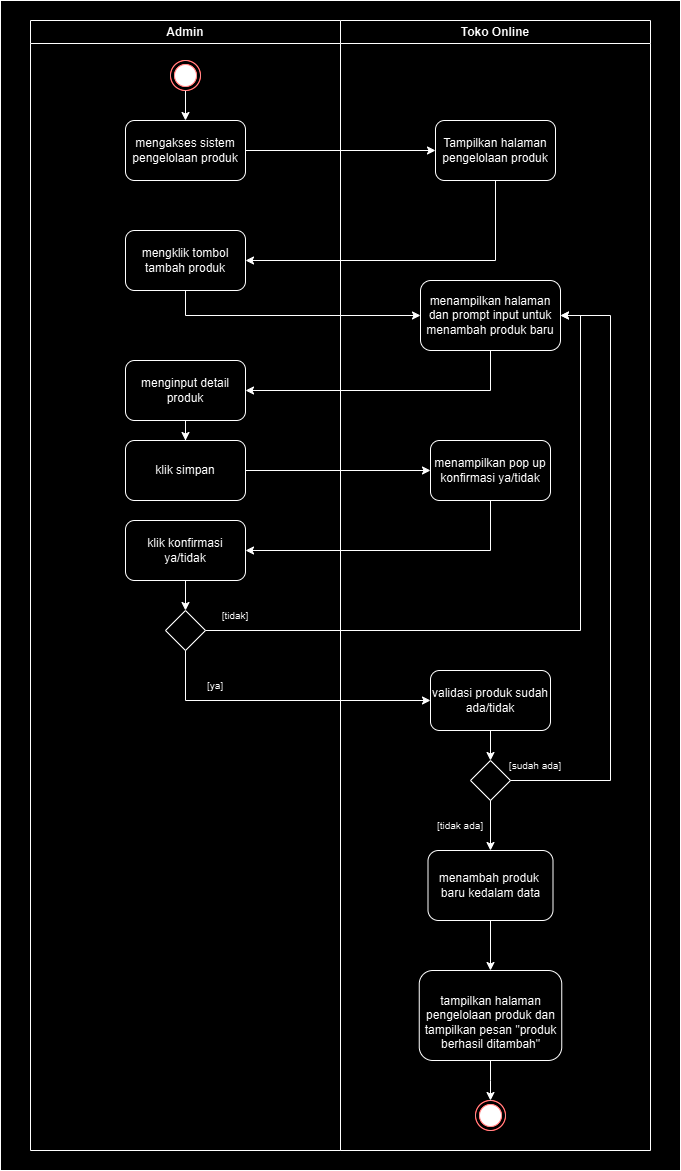
\includegraphics[width=0.7\textwidth]{images/avtivitymenambahsepatudiagram.png}
    \captionsetup{justification=centering}
    \caption{\textit{Activity Diagram Menambah Sepatu}}
    \label{fig:activity-recommendation}
\end{figure}

\begin{figure}[H]
    \centering
    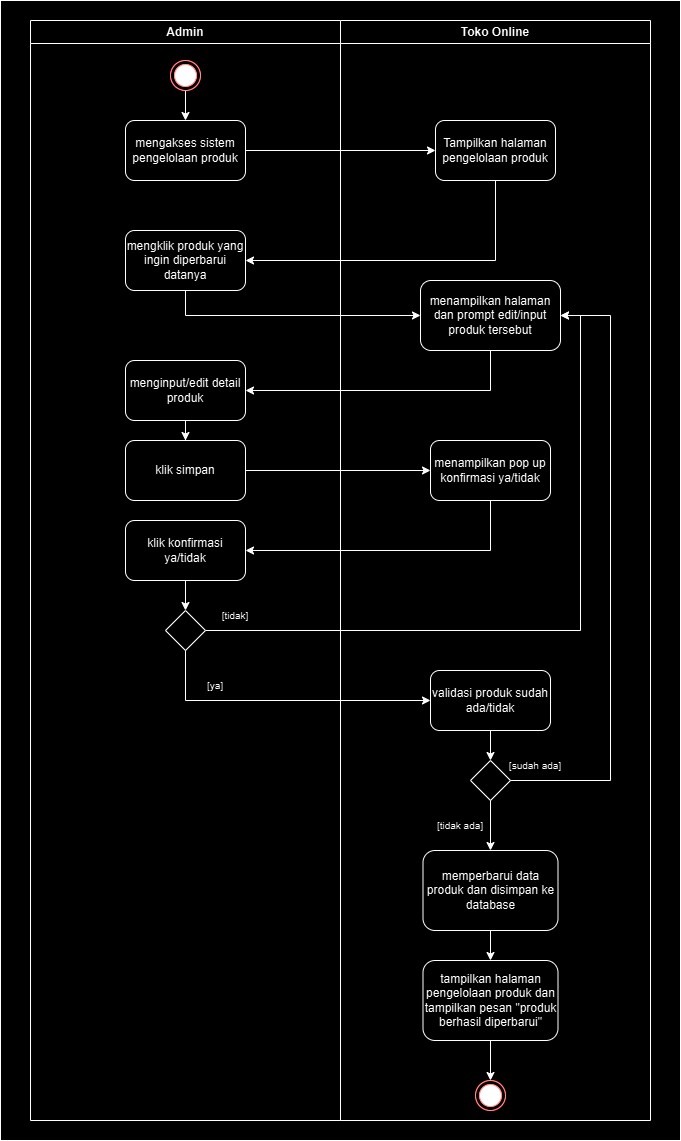
\includegraphics[width=0.7\textwidth]{images/activityupdatesepatudiagram.png}
    \captionsetup{justification=centering}
    \caption{\textit{Activity Diagram Update Sepatu}}
    \label{fig:activity-admin}
\end{figure}

\section{Project Documentation}

\subsection{Implementation}

\begin{itemize}
    \item \textbf{Analisis Kebutuhan Detail}:
    \begin{itemize}
        \item Menganalisis pola belanja online pengguna untuk mengidentifikasi area yang dapat dioptimalkan
        \item Menentukan fitur-fitur utama yang diperlukan dalam sistem rekomendasi
        \item Mengidentifikasi teknologi yang sesuai untuk pengembangan platform
    \end{itemize}

    \item \textbf{Pengembangan \& Pengujian Sistem}:
    \begin{itemize}
        \item Membangun frontend menggunakan React.js untuk antarmuka yang responsif
        \item Mengembangkan backend dengan Flask dan mengintegrasikan sistem rekomendasi NMF
        \item Melakukan pengujian untuk memastikan akurasi rekomendasi dan kinerja sistem
    \end{itemize}

    \item \textbf{Integrasi Sistem E-commerce}:
    \begin{itemize}
        \item Mengintegrasikan sistem rekomendasi dengan katalog produk
        \item Memastikan sistem pembayaran dan keranjang belanja berfungsi dengan baik
        \item Mengoptimalkan performa sistem secara keseluruhan
    \end{itemize}
\end{itemize}

\subsection{Results and Discussion}
\subsubsection{Hasil Evaluasi Model}
\begin{itemize}
    \item \textit{Gambar Evaluasi Metrik}:
    \begin{itemize}
        \item 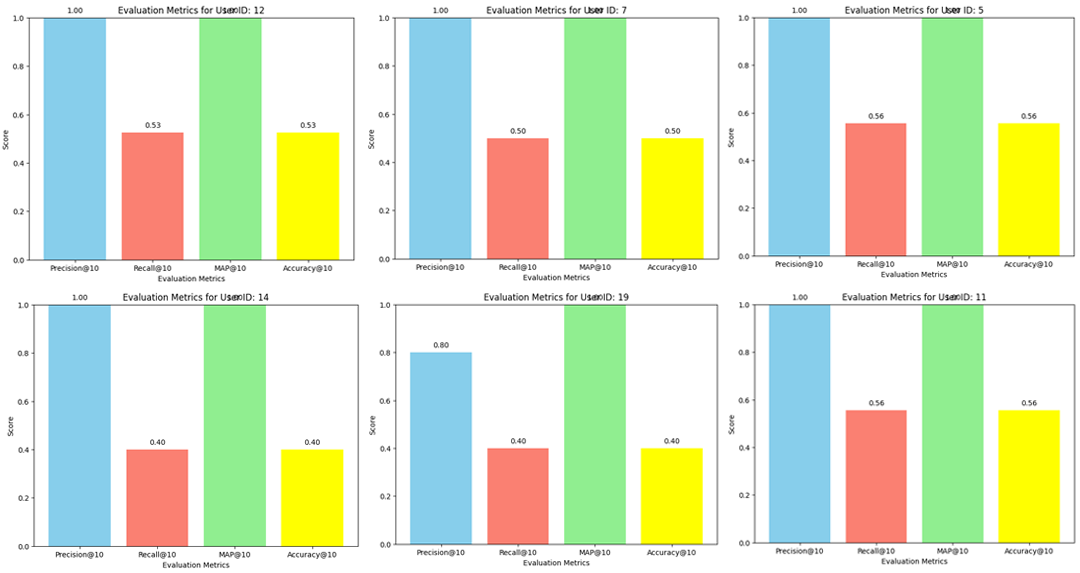
\includegraphics[width=0.6\textwidth]{images/Tabel.png}
        \item \textbf{Evaluation Metrics untuk User ID 12}:
        \begin{itemize}
            \item \textit{Precision@10}: 1.0
            \item \textit{Recall@10}: 0.53
            \item \textit{MAP@10}: 1.0
            \item \textit{Accuracy@10}: 0.53
        \end{itemize}
        \item \textbf{Evaluation Metrics untuk User ID 7}:
        \begin{itemize}
            \item \textit{Precision@10}: 1.0
            \item \textit{Recall@10}: 0.5
            \item \textit{MAP@10}: 1.0
            \item \textit{Accuracy@10}: 0.5
        \end{itemize}
        \item \textbf{Evaluation Metrics untuk User ID 5}:
        \begin{itemize}
            \item \textit{Precision@10}: 1.0
            \item \textit{Recall@10}: 0.56
            \item \textit{MAP@10}: 1.0
            \item \textit{Accuracy@10}: 0.56
        \end{itemize}
        \item \textbf{Evaluation Metrics untuk User ID 14}:
        \begin{itemize}
            \item \textit{Precision@10}: 1.0
            \item \textit{Recall@10}: 0.4
            \item \textit{MAP@10}: 1.0
            \item \textit{Accuracy@10}: 0.4
        \end{itemize}
        \item \textbf{Evaluation Metrics untuk User ID 19}:
        \begin{itemize}
            \item \textit{Precision@10}: 0.8
            \item \textit{Recall@10}: 0.4
            \item \textit{MAP@10}: 1.0
            \item \textit{Accuracy@10}: 0.4
        \end{itemize}
        \item \textbf{Evaluation Metrics untuk User ID 11}:
        \begin{itemize}
            \item \textit{Precision@10}: 1.0
            \item \textit{Recall@10}: 0.56
            \item \textit{MAP@10}: 1.0
            \item \textit{Accuracy@10}: 0.56
        \end{itemize}
    \end{itemize}
    
    \item \textit{Simpulan}:
    \begin{itemize}
        \item Setiap modul pengguna menunjukkan variasi dalam metrik evaluasi, yang mencerminkan perbedaan dalam pola interaksi dan preferensi pengguna.
        \item Pengguna dengan riwayat interaksi yang lebih kaya cenderung memiliki nilai precision dan recall yang lebih tinggi, menunjukkan bahwa model dapat memberikan rekomendasi yang lebih akurat.
        \item Variasi dalam MAP dan accuracy menunjukkan bahwa meskipun model memberikan rekomendasi yang relevan, ada ruang untuk peningkatan dalam menangkap semua item relevan.
    \end{itemize}
\subsubsection{Discussion}

Website e-commerce R\&R dengan sistem rekomendasi telah berhasil diimplementasikan dan menunjukkan hasil yang menjanjikan. Sistem ini dibangun menggunakan dataset yang terdiri dari 50 produk sepatu yang terbagi dalam 5 kategori utama: formal, sport, heels, boots, dan casual. Setiap kategori memiliki 10 jenis sepatu yang berbeda, memberikan variasi yang cukup untuk pengujian sistem rekomendasi.

Implementasi algoritma Non-negative Matrix Factorization (NMF) terbukti efektif dalam mengidentifikasi pola laten dari data interaksi pengguna. Model ini berhasil menganalisis berbagai jenis interaksi seperti view, wishlist, cart, dan purchase untuk menghasilkan rekomendasi yang dipersonalisasi. Untuk pengguna yang telah memiliki riwayat interaksi, sistem mampu memberikan rekomendasi yang lebih akurat dan relevan dengan preferensi mereka. Sementara itu, untuk mengatasi cold start problem pada pengguna baru, sistem menerapkan pendekatan hybrid dengan menggabungkan rekomendasi berbasis popularitas.

Dari segi antarmuka pengguna, website berhasil mengintegrasikan sistem rekomendasi dengan tampilan yang responsif menggunakan React.js. Halaman utama dirancang dengan layout yang intuitif, menampilkan berbagai kategori produk dan rekomendasi yang dipersonalisasi. Proses autentikasi pengguna dibuat sederhana namun tetap memperhatikan aspek keamanan. Halaman katalog dan detail produk menyajikan informasi yang komprehensif, memudahkan pengguna dalam mengambil keputusan pembelian.

Meskipun sistem menunjukkan performa yang baik, beberapa tantangan masih perlu diatasi. Keterbatasan dataset dengan hanya 50 produk mempengaruhi keragaman rekomendasi yang dapat diberikan. Cold start problem, terutama untuk pengguna baru, masih menjadi tantangan meskipun telah dimitigasi dengan pendekatan hybrid. Selain itu, variasi dalam metrik evaluasi seperti MAP dan accuracy menunjukkan bahwa masih ada ruang untuk peningkatan dalam menangkap semua item yang relevan.

Secara keseluruhan, implementasi sistem rekomendasi pada platform e-commerce R\&R telah berhasil meningkatkan pengalaman berbelanja pengguna dengan memberikan rekomendasi yang relevan dan dipersonalisasi. Untuk pengembangan ke depan, peningkatan jumlah dataset dan penyempurnaan algoritma akan menjadi fokus utama untuk meningkatkan akurasi dan relevansi rekomendasi lebih lanjut.\end{itemize}
  

% ... existing code ...




\subsection{Conclusion}

Website e-commerce sepatu R\&R dengan sistem rekomendasi berbasis machine learning telah berhasil dikembangkan dan diimplementasikan dengan hasil yang menjanjikan. Dengan memanfaatkan algoritma Non-negative Matrix Factorization (NMF), platform ini mampu menganalisis pola interaksi pengguna seperti view, wishlist, cart, dan pembelian untuk memberikan rekomendasi produk yang dipersonalisasi. Sistem ini tidak hanya memudahkan pengguna dalam menemukan sepatu yang sesuai dengan preferensi mereka, tetapi juga meningkatkan efisiensi dalam proses pencarian produk.

Melalui integrasi teknologi modern seperti React.js untuk frontend dan Flask untuk backend, platform ini menyajikan antarmuka yang responsif dan pengalaman pengguna yang optimal. Hasil evaluasi menunjukkan performa yang baik dengan nilai Precision@10 rata-rata mencapai 0.96 dan MAP@10 yang konsisten mencapai 1.0, mengindikasikan akurasi yang tinggi dalam memberikan rekomendasi yang relevan. Meskipun terdapat variasi dalam nilai Recall@10 yang berkisar antara 0.4 hingga 0.56, hal ini menunjukkan bahwa model masih memiliki ruang untuk peningkatan dalam menangkap semua item yang relevan.

Platform ini berhasil mengatasi tantangan umum dalam sistem rekomendasi e-commerce, seperti cold start problem, dengan mengadopsi pendekatan hybrid yang menggabungkan rekomendasi berbasis popularitas untuk pengguna baru. Meskipun demikian, keterbatasan dataset yang hanya mencakup 50 produk sepatu mempengaruhi keragaman rekomendasi yang dapat diberikan. Untuk pengembangan ke depan, peningkatan jumlah dataset dan penyempurnaan algoritma akan menjadi fokus utama untuk meningkatkan akurasi dan relevansi rekomendasi.

Secara keseluruhan, implementasi sistem rekomendasi pada platform e-commerce R\&R telah berhasil menciptakan pengalaman berbelanja yang lebih personal dan efisien. Dengan mengotomatisasi proses rekomendasi produk berdasarkan preferensi pengguna, platform ini tidak hanya meningkatkan kepuasan pelanggan tetapi juga berpotensi meningkatkan konversi penjualan. Keberhasilan ini menunjukkan bahwa integrasi teknologi machine learning dalam e-commerce dapat memberikan nilai tambah yang signifikan dalam meningkatkan pengalaman berbelanja online.

\section{Appendices (if applicable)}
\begin{figure}[H]
    \centering
    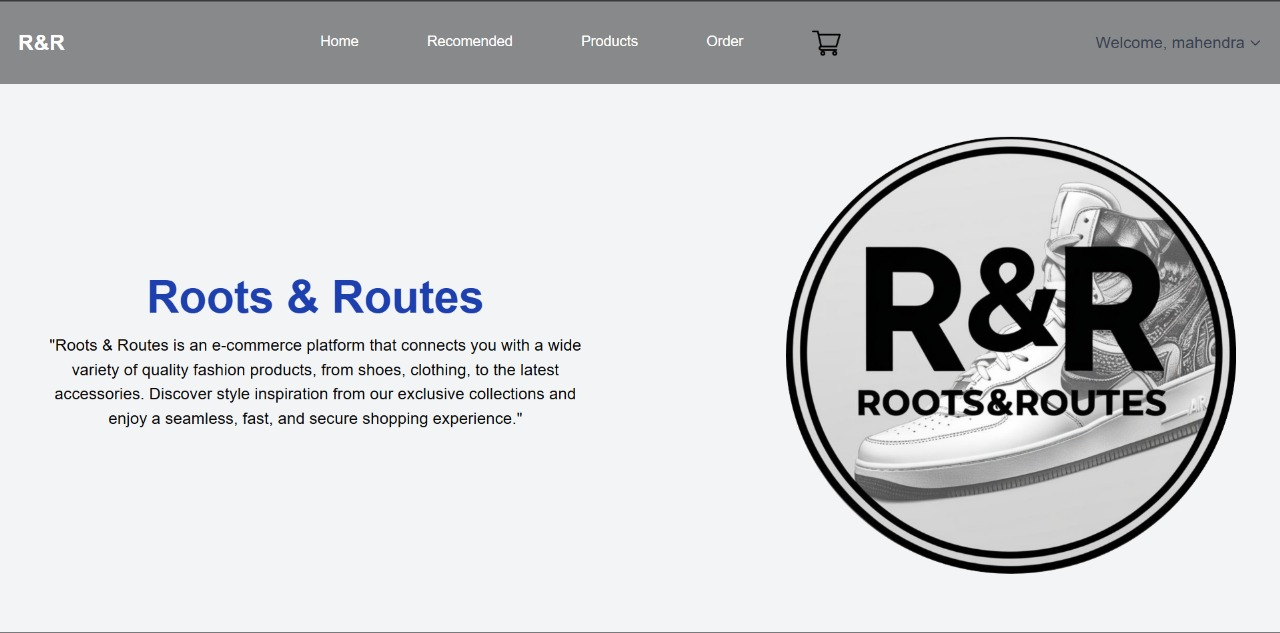
\includegraphics[width=0.7\textwidth]{images/Homepage.jpeg}
    \captionsetup{justification=centering}
    \caption{\textit{Homopage}}
    \label{fig:activity-login}
\end{figure}
\begin{figure}[H]
    \centering
    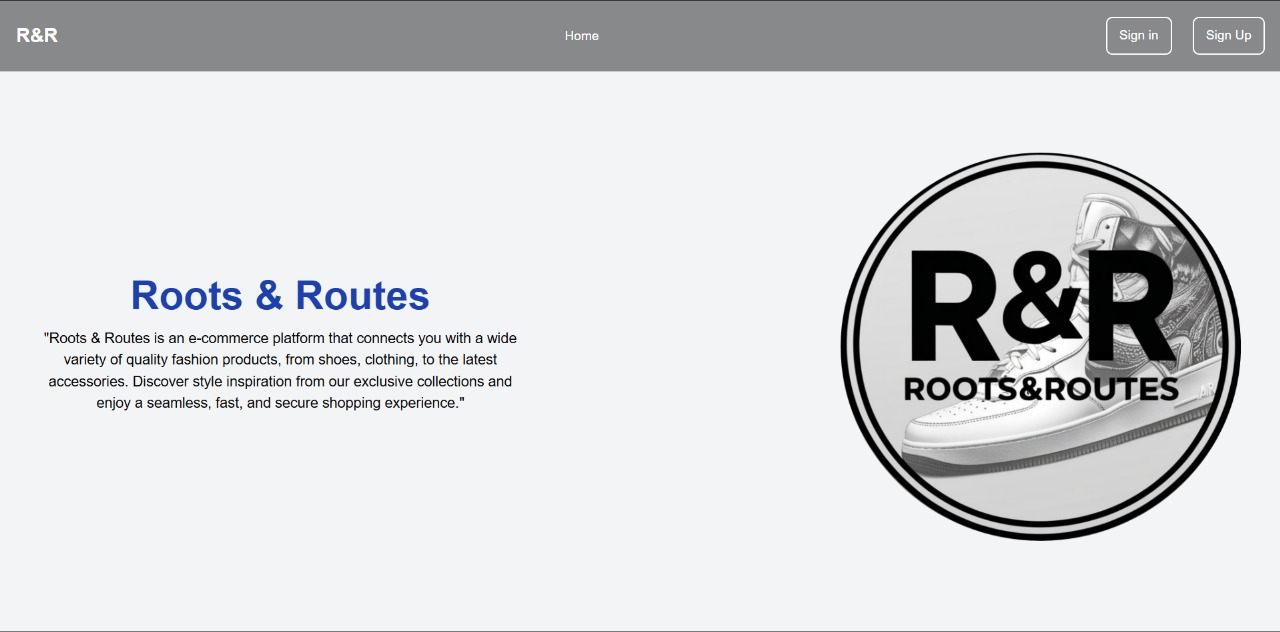
\includegraphics[width=0.7\textwidth]{images/homepageNoLogin.jpeg}
    \captionsetup{justification=centering}
    \caption{\textit{Homepage Tanpa Login}}
    \label{fig:activity-login}
\end{figure}
\begin{figure}[H]
    \centering
    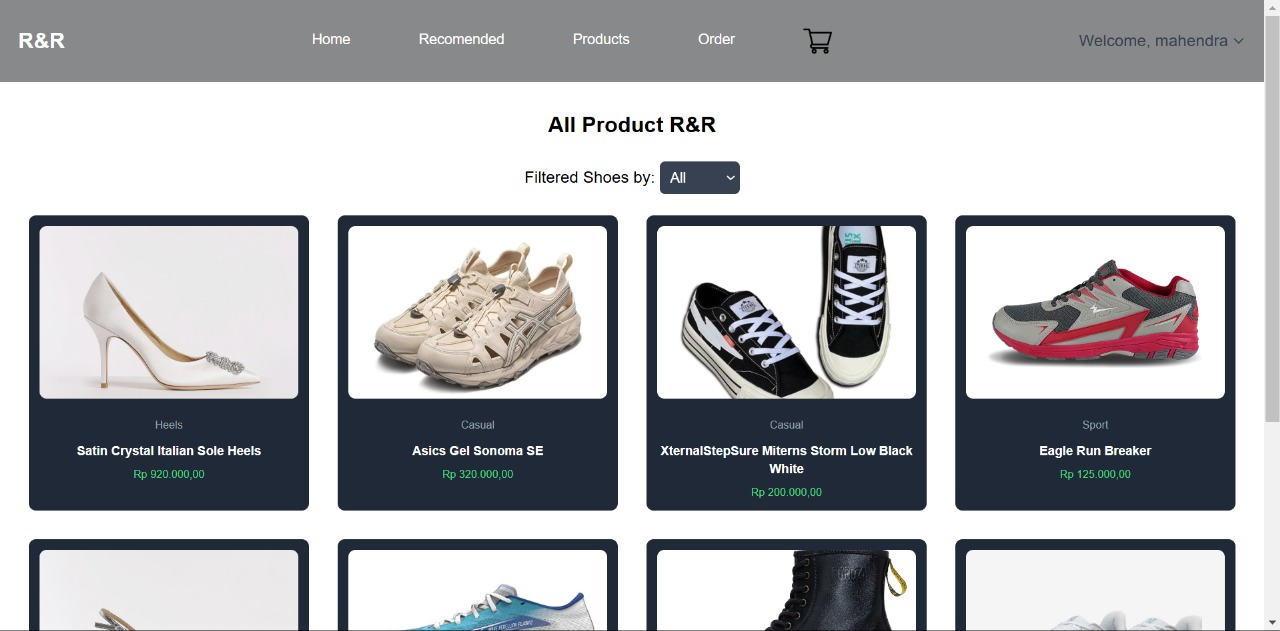
\includegraphics[width=0.7\textwidth]{images/productPage.jpeg}
    \captionsetup{justification=centering}
    \caption{\textit{Product Page}}
    \label{fig:activity-login}
\end{figure}
\begin{figure}[H]
    \centering
    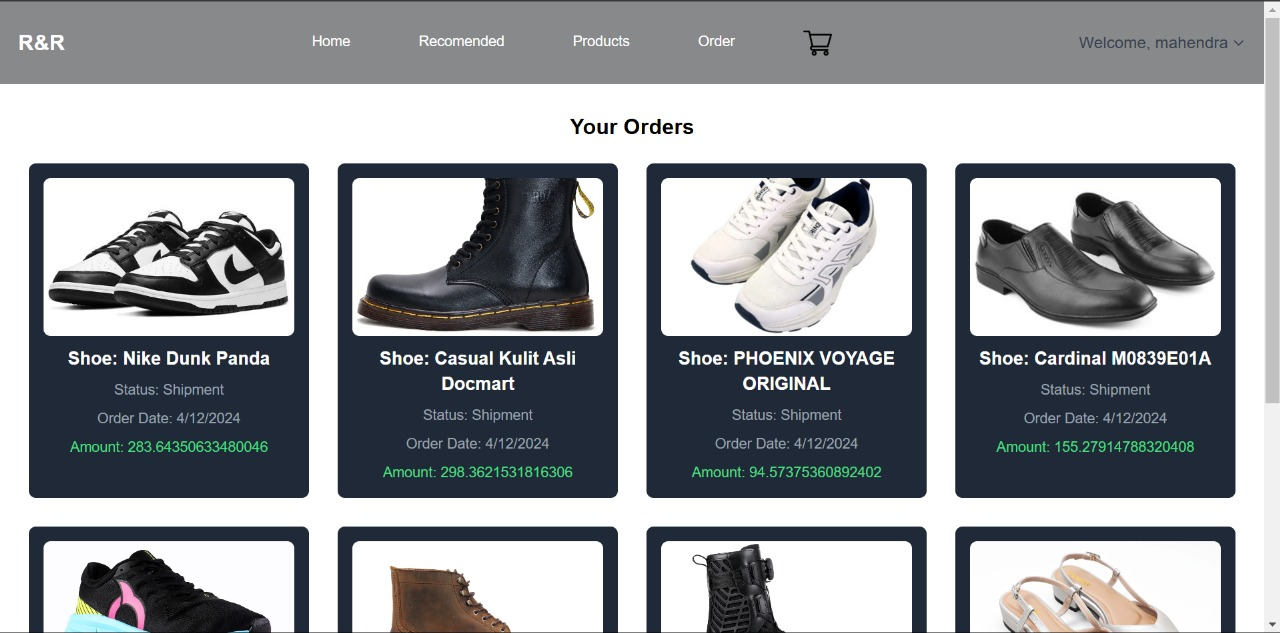
\includegraphics[width=0.7\textwidth]{images/orderPage.jpeg}
    \captionsetup{justification=centering}
    \caption{\textit{Order Page}}
    \label{fig:activity-login}
\end{figure}
\begin{figure}[H]
    \centering
    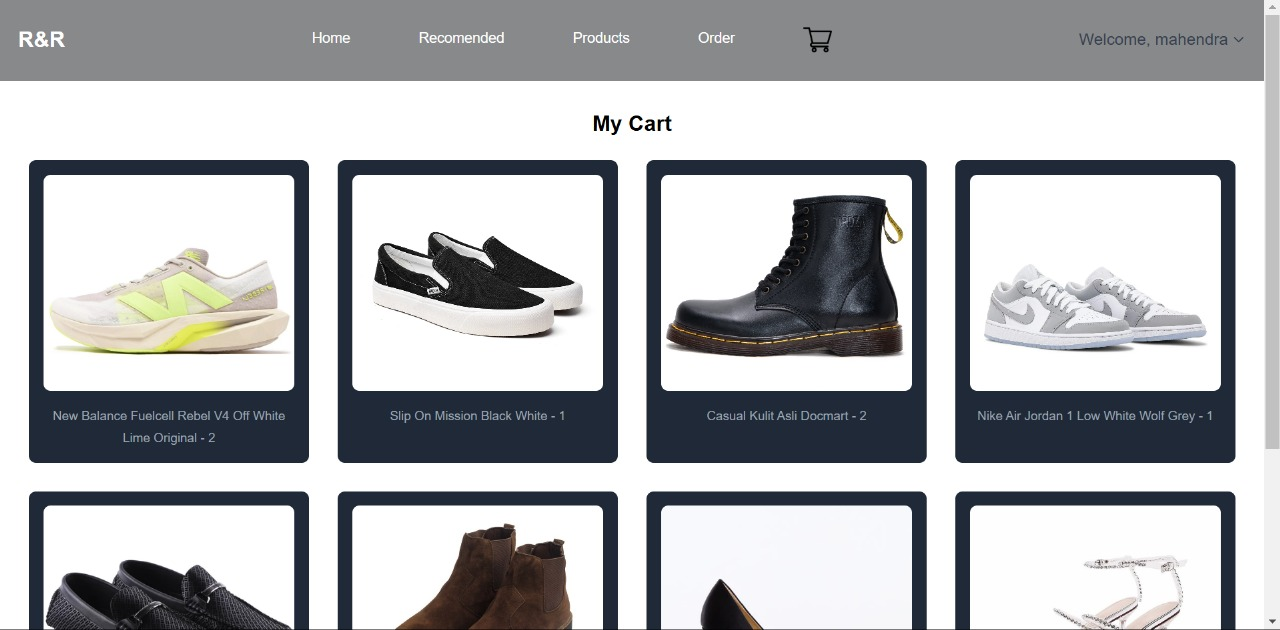
\includegraphics[width=0.7\textwidth]{images/cartPage.jpeg}
    \captionsetup{justification=centering}
    \caption{\textit{Cart Page}}
    \label{fig:activity-login}
\end{figure}
\begin{figure}[H]
    \centering
    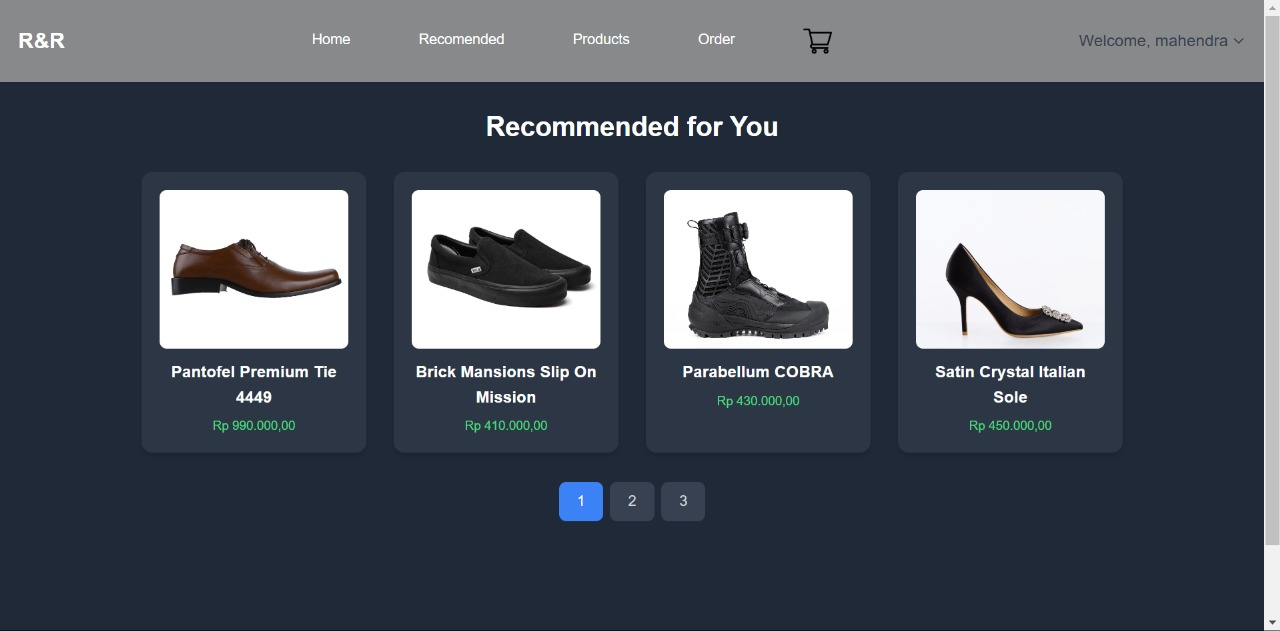
\includegraphics[width=0.7\textwidth]{images/recommendedPage.jpeg}
    \captionsetup{justification=centering}
    \caption{\textit{Recommended Page}}
    \label{fig:activity-login}
\end{figure}
\begin{figure}[H]
    \centering
    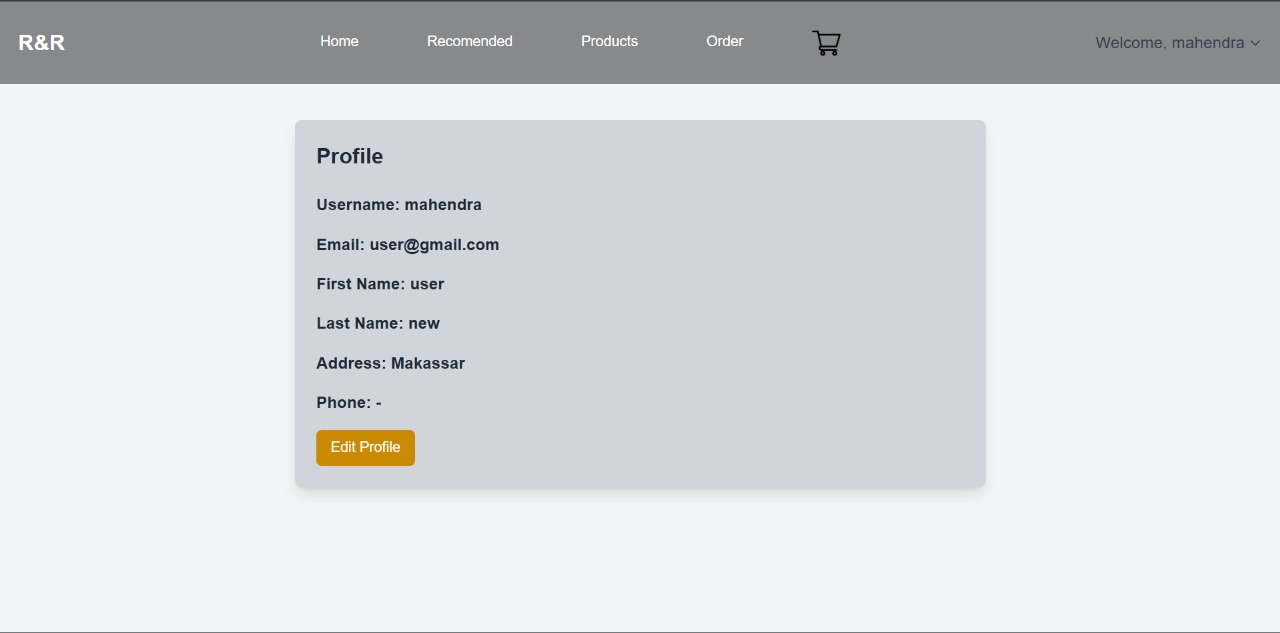
\includegraphics[width=0.7\textwidth]{images/profilePage.jpeg}
    \captionsetup{justification=centering}
    \caption{\textit{Profile Page}}
    \label{fig:activity-login}
\end{figure}
\begin{figure}[H]
    \centering
    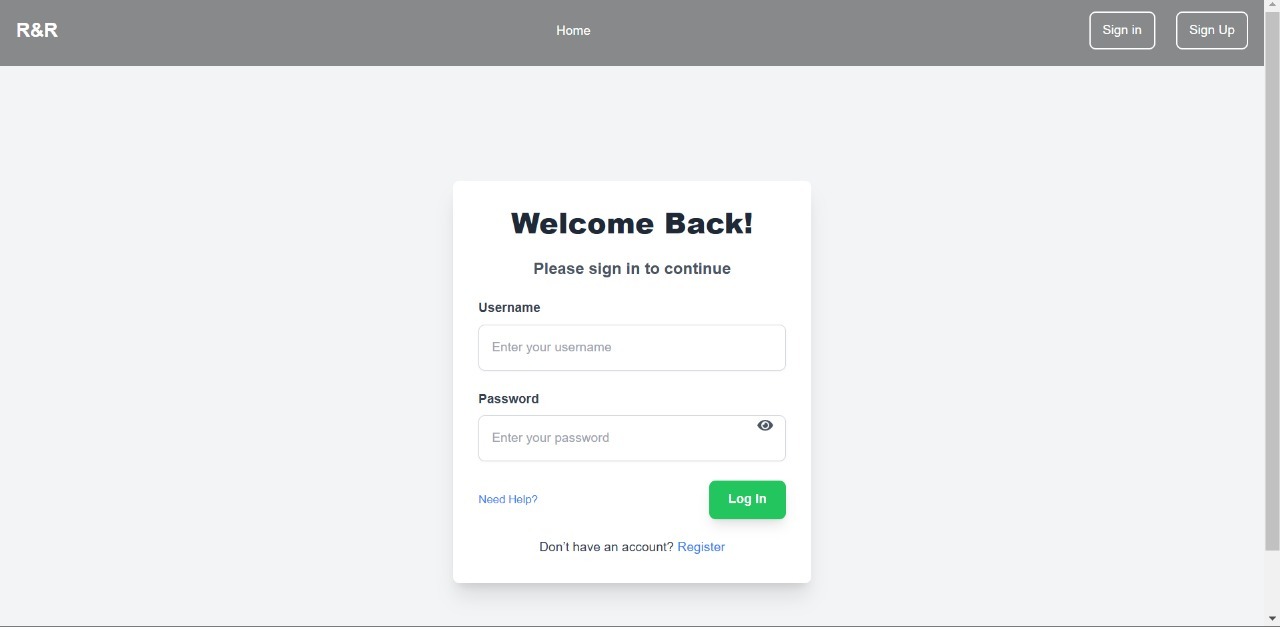
\includegraphics[width=0.7\textwidth]{images/signinPage.jpeg}
    \captionsetup{justification=centering}
    \caption{\textit{Signin Page}}
    \label{fig:activity-login}
\end{figure}
\begin{figure}[H]
    \centering
    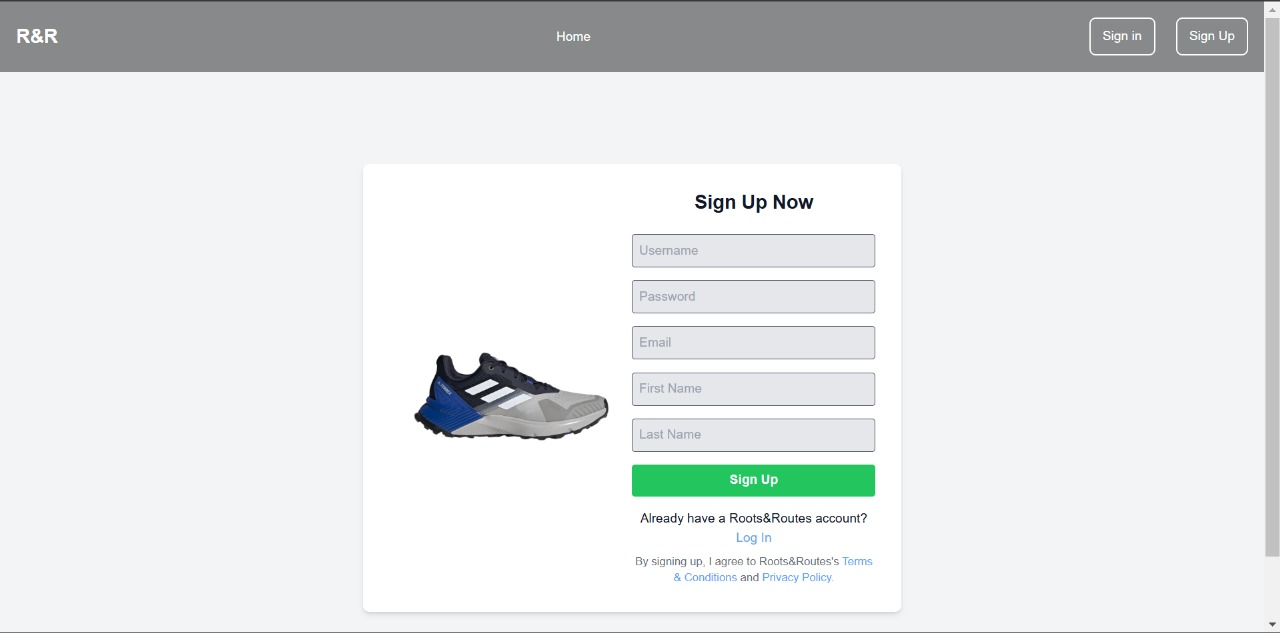
\includegraphics[width=0.7\textwidth]{images/signupPage.jpeg}
    \captionsetup{justification=centering}
    \caption{\textit{Signup Page}}
    \label{fig:activity-login}
\end{figure}
\begin{figure}[H]
    \centering
    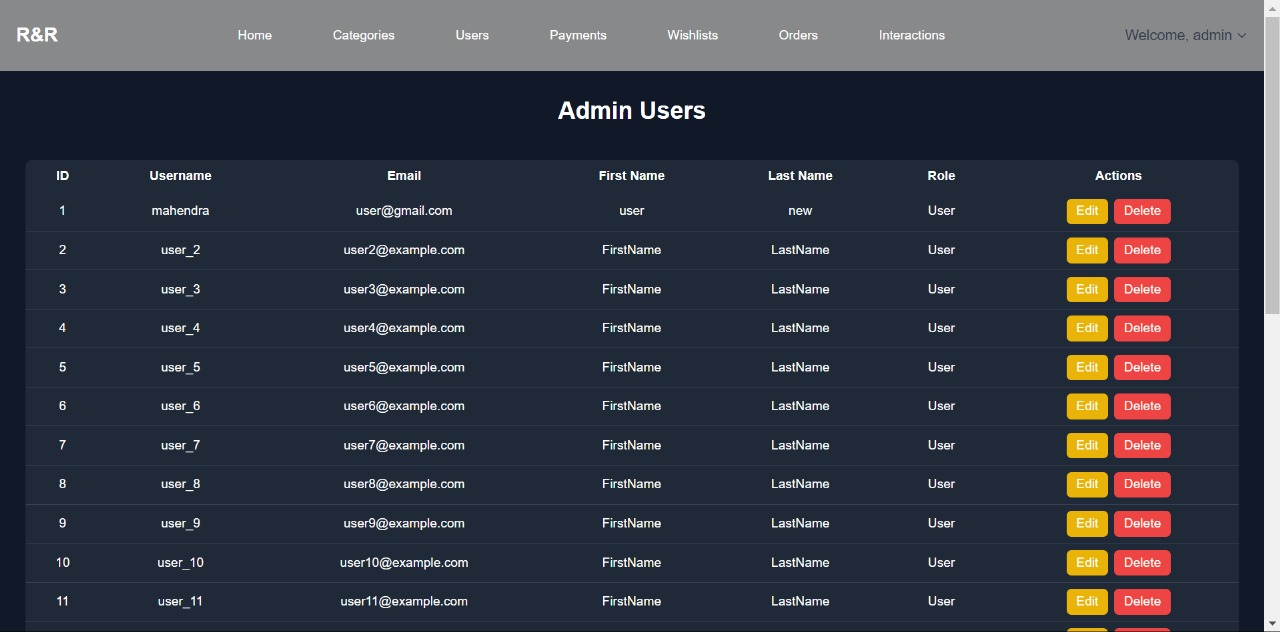
\includegraphics[width=0.7\textwidth]{images/userPageAdmin.jpeg}
    \captionsetup{justification=centering}
    \caption{\textit{User Admin Page}}
    \label{fig:activity-login}
\end{figure}
\begin{figure}[H]
    \centering
    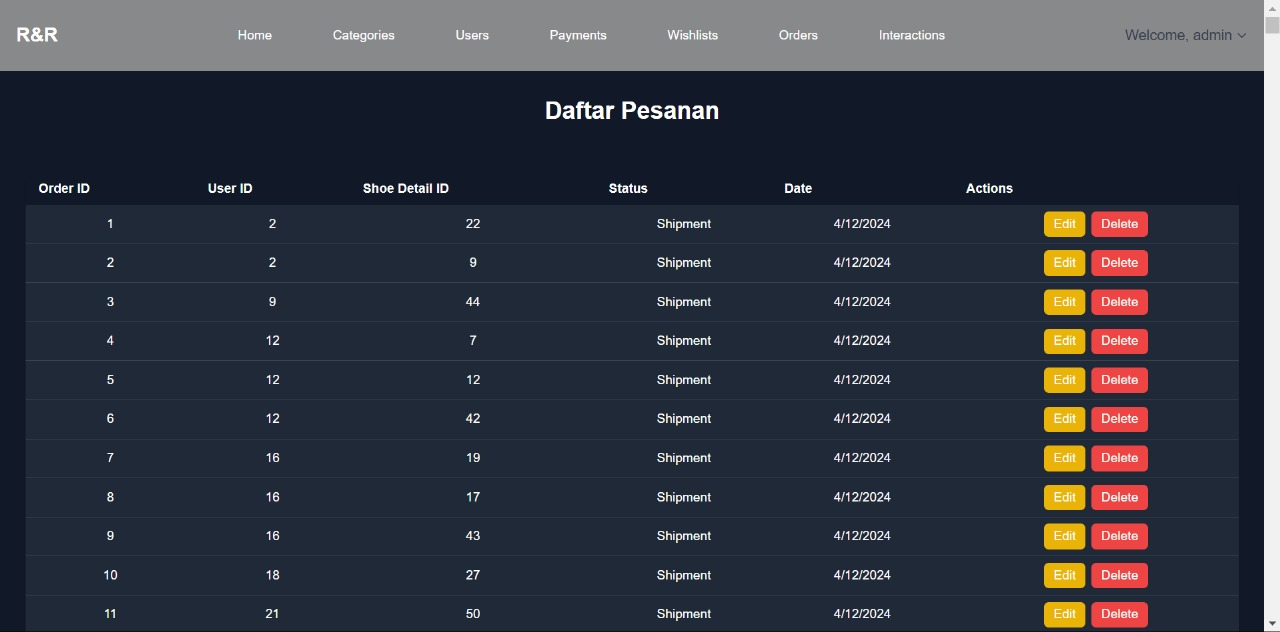
\includegraphics[width=0.7\textwidth]{images/orderPageAdmin.jpeg}
    \captionsetup{justification=centering}
    \caption{\textit{Order Admin Page}}
    \label{fig:activity-login}
\end{figure}
\begin{figure}[H]
    \centering
    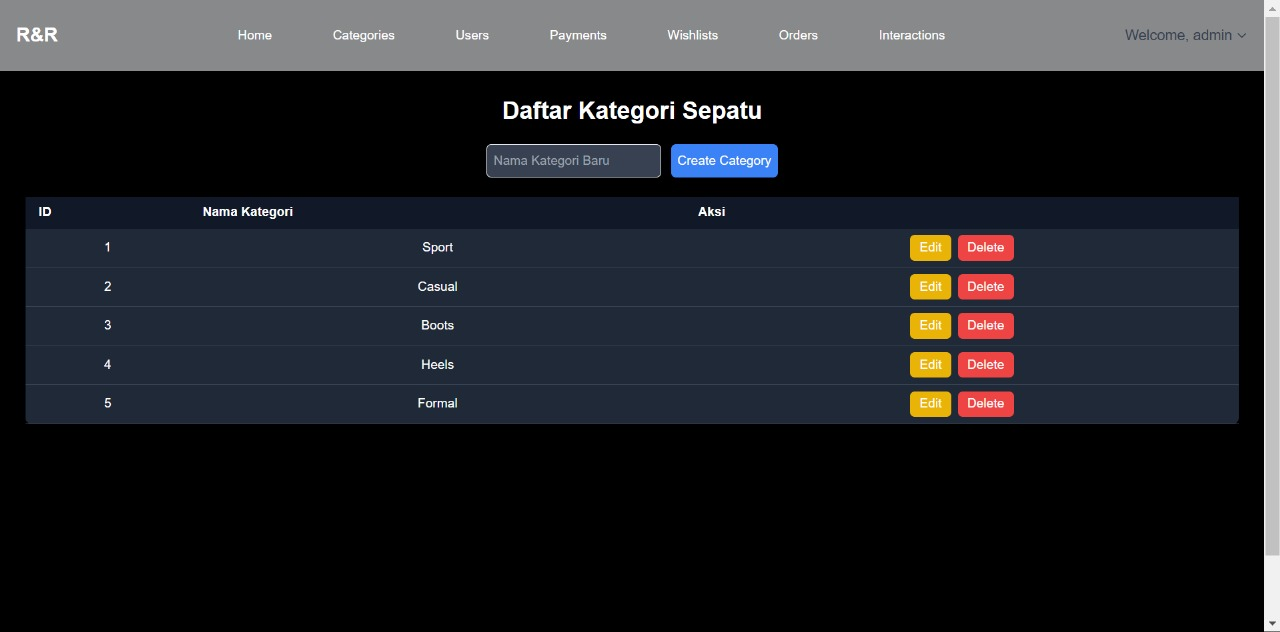
\includegraphics[width=0.7\textwidth]{images/categoriesPageAdmin.jpeg}
    \captionsetup{justification=centering}
    \caption{\textit{Categories Admin Page}}
    \label{fig:activity-login}
\end{figure}
\begin{figure}[H]
    \centering
    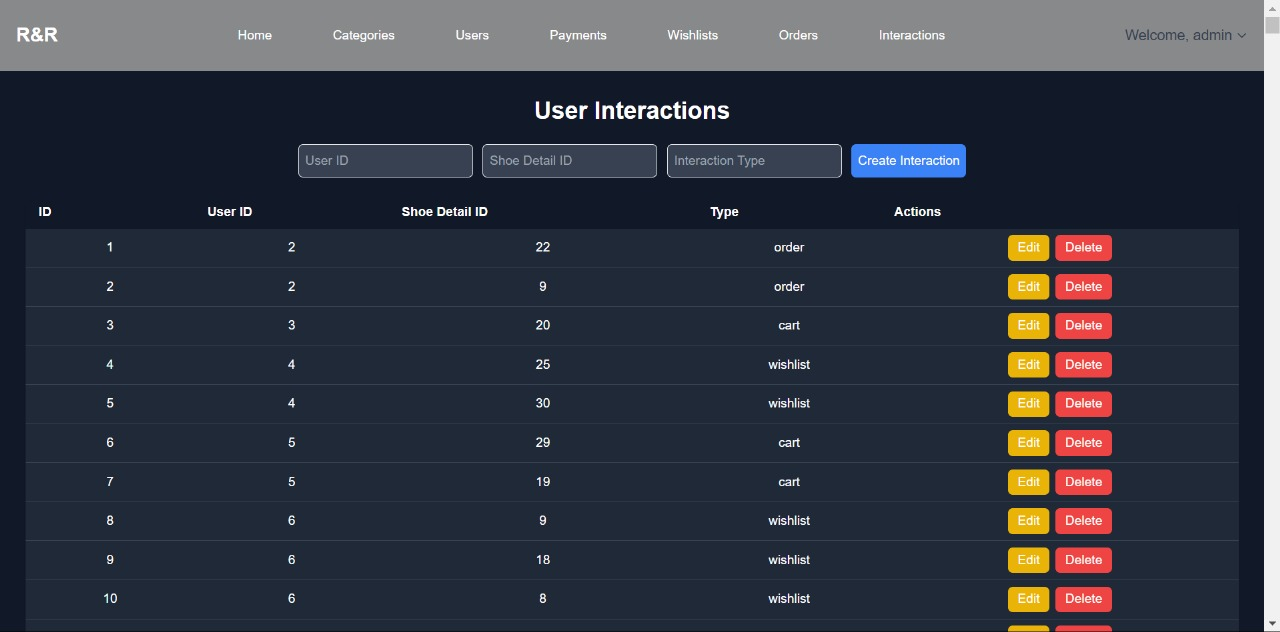
\includegraphics[width=0.7\textwidth]{images/userInteractionPageAdmin.jpeg}
    \captionsetup{justification=centering}
    \caption{\textit{User Interaction Admin Page}}
    \label{fig:activity-login}
\end{figure}



\end{document}